%%%%%%%%%%%%%%%%%%%%%%%%%%%%%%%%%%%%%%%%%%%%%%%%%%%%%%%%%%%%%%%%%%%%%
%%                                                                 %%
%% Please do not use \input{...} to include other tex files.       %%
%% Submit your LaTeX manuscript as one .tex document.              %%
%%                                                                 %%
%% All additional figures and files should be attached             %%
%% separately and not embedded in the \TeX\ document itself.       %%
%%                                                                 %%
%%%%%%%%%%%%%%%%%%%%%%%%%%%%%%%%%%%%%%%%%%%%%%%%%%%%%%%%%%%%%%%%%%%%%

%%\documentclass[referee,sn-basic]{sn-jnl}% referee option is meant for double line spacing

%%=======================================================%%
%% to print line numbers in the margin use lineno option %%
%%=======================================================%%

%%\documentclass[lineno,sn-basic]{sn-jnl}% Basic Springer Nature Reference Style/Chemistry Reference Style

%%======================================================%%
%% to compile with pdflatex/xelatex use pdflatex option %%
%%======================================================%%

%%\documentclass[pdflatex,sn-basic]{sn-jnl}% Basic Springer Nature Reference Style/Chemistry Reference Style

%%\documentclass[sn-basic]{sn-jnl}% Basic Springer Nature Reference Style/Chemistry Reference Style
\documentclass[sn-mathphys,Numbered]{sn-jnl}% Math and Physical Sciences Reference Style
%%\documentclass[sn-aps]{sn-jnl}% American Physical Society (APS) Reference Style
%%\documentclass[sn-vancouver]{sn-jnl}% Vancouver Reference Style
%%\documentclass[sn-apa]{sn-jnl}% APA Reference Style
%%\documentclass[sn-chicago]{sn-jnl}% Chicago-based Humanities Reference Style
%%\documentclass[sn-standardnature]{sn-jnl}% Standard Nature Portfolio Reference Style
%%\documentclass[default]{sn-jnl}% Default
%%\documentclass[default,iicol]{sn-jnl}% Default with double column layout

%%%% Standard Packages
%%<additional latex packages if required can be included here>
%%%%

%%%%%=============================================================================%%%%
%%%%  Remarks: This template is provided to aid authors with the preparation
%%%%  of original research articles intended for submission to journals published 
%%%%  by Springer Nature. The guidance has been prepared in partnership with 
%%%%  production teams to conform to Springer Nature technical requirements. 
%%%%  Editorial and presentation requirements differ among journal portfolios and 
%%%%  research disciplines. You may find sections in this template are irrelevant 
%%%%  to your work and are empowered to omit any such section if allowed by the 
%%%%  journal you intend to submit to. The submission guidelines and policies 
%%%%  of the journal take precedence. A detailed User Manual is available in the 
%%%%  template package for technical guidance.
%%%%%=============================================================================%%%%

\jyear{2021}%

%% as per the requirement new theorem styles can be included as shown below
\theoremstyle{thmstyleone}%
\newtheorem{theorem}{Theorem}%  meant for continuous numbers
%%\newtheorem{theorem}{Theorem}[section]% meant for sectionwise numbers
%% optional argument [theorem] produces theorem numbering sequence instead of independent numbers for Proposition
\newtheorem{proposition}[theorem]{Proposition}% 
%%\newtheorem{proposition}{Proposition}% to get separate numbers for theorem and proposition etc.

\theoremstyle{thmstyletwo}%
\newtheorem{example}{Example}%
\newtheorem{remark}{Remark}%

\theoremstyle{thmstylethree}%
\newtheorem{definition}{Definition}%

\raggedbottom
%%\unnumbered% uncomment this for unnumbered level heads

%% My used library
\usepackage{csquotes}
\usepackage{subcaption}
\usepackage{graphicx, adjustbox}
\usepackage{caption}
\usepackage{enumitem}
\usepackage{float}
\usepackage{longtable,booktabs,array}
\graphicspath{{Figs}{Figs/}}

\begin{document}

\title[Article Title]{Exploratory analysis of suicidal intensity within depression, dissect social media post}

%%=============================================================%%
%% Prefix	-> \pfx{Dr}
%% GivenName	-> \fnm{Joergen W.}
%% Particle	-> \spfx{van der} -> surname prefix
%% FamilyName	-> \sur{Ploeg}
%% Suffix	-> \sfx{IV}
%% NatureName	-> \tanm{Poet Laureate} -> Title after name
%% Degrees	-> \dgr{MSc, PhD}
%% \author*[1,2]{\pfx{Dr} \fnm{Joergen W.} \spfx{van der} \sur{Ploeg} \sfx{IV} \tanm{Poet Laureate} 
%%                 \dgr{MSc, PhD}}\email{iauthor@gmail.com}
%%=============================================================%%

\author*[1,2]{\fnm{Md Iftekharul} \sur{Mobin}}\email{iftekhar.mobin@gmail.com}

\author[2,3]{\fnm{Second} \sur{Author}}\email{iiauthor@gmail.com}
\equalcont{These authors contributed equally to this work.}

\author[1,2]{\fnm{Third} \sur{Author}}\email{iiiauthor@gmail.com}
\equalcont{These authors contributed equally to this work.}

\affil*[1]{\orgdiv{Department}, \orgname{Organization}, \orgaddress{\street{Street}, \city{City}, \postcode{100190}, \state{State}, \country{Country}}}

\affil[2]{\orgdiv{Department}, \orgname{Organization}, \orgaddress{\street{Street}, \city{City}, \postcode{10587}, \state{State}, \country{Country}}}

\affil[3]{\orgdiv{Department}, \orgname{Organization}, \orgaddress{\street{Street}, \city{City}, \postcode{610101}, \state{State}, \country{Country}}}

%%==================================%%
%% sample for unstructured abstract %%
%%==================================%%

\abstract{This study uses Reddit's social media datasets for exploratory data analysis to estimate the degree of suicidal thoughts within depressed person's post. The objective is to determine if a depressed individual has a suicidal tendency, determine the degree of the intensity or the opposite. This study presents an unsupervised feature analysis using the LDA topic model of the Reddit C-SSRS dataset followed by supervised classification to quantize significance. Latent suicidal intents, cross-topic co-occurrence patterns, and dominant high-impact keywords of suicide are revealed from unsupervised LDA modeling. Furthermore, Supervised machine learning classifier models are applied to determine the severity of suicide tendencies. To get the best results, cutting edge tex embedding vectorization techniques and machine learning estimators are applied. Statistical measurements depicts the degree of suicide intensity within depressed label post. From the analysis it is revealed that suicidal tendency within depression people post is extremely high. Depressed person's post showed 60\% similarities in various categories of suicidal intensity.}

%%================================%%
%% Sample for structured abstract %%
%%================================%%

% \abstract{\textbf{Purpose:} The abstract serves both as a general introduction to the topic and as a brief, non-technical summary of the main results and their implications. The abstract must not include subheadings (unless expressly permitted in the journal's Instructions to Authors), equations or citations. As a guide the abstract should not exceed 200 words. Most journals do not set a hard limit however authors are advised to check the author instructions for the journal they are submitting to.
% 
% \textbf{Methods:} The abstract serves both as a general introduction to the topic and as a brief, non-technical summary of the main results and their implications. The abstract must not include subheadings (unless expressly permitted in the journal's Instructions to Authors), equations or citations. As a guide the abstract should not exceed 200 words. Most journals do not set a hard limit however authors are advised to check the author instructions for the journal they are submitting to.
% 
% \textbf{Results:} The abstract serves both as a general introduction to the topic and as a brief, non-technical summary of the main results and their implications. The abstract must not include subheadings (unless expressly permitted in the journal's Instructions to Authors), equations or citations. As a guide the abstract should not exceed 200 words. Most journals do not set a hard limit however authors are advised to check the author instructions for the journal they are submitting to.
% 
% \textbf{Conclusion:} The abstract serves both as a general introduction to the topic and as a brief, non-technical summary of the main results and their implications. The abstract must not include subheadings (unless expressly permitted in the journal's Instructions to Authors), equations or citations. As a guide the abstract should not exceed 200 words. Most journals do not set a hard limit however authors are advised to check the author instructions for the journal they are submitting to.}

\keywords{Suicide and Depression, NLP, Unsupervised LDA model, exploratory analysis, feature extraction}

%%\pacs[JEL Classification]{D8, H51}
%%\pacs[MSC Classification]{35A01, 65L10, 65L12, 65L20, 65L70}

\maketitle

\section{Introduction}\label{sec1}
Suicide is a major cause of death globally. In india, USA and many other countries large number of population dies because of suicide \cite{havigerova2019text, singh2022startling}. Only In USA approximately 46,000 people committed suicide in 2020 \cite{singh2022startling}. Depression and suicide this two phenomenon are closely connected with each other. Depression triggers suicidal risk. Several studies showed that depression patients are very prone to suicidal attempt \cite{vuorilehto2006suicidal, mcgirr2007examination, hawton2013risk}. According to \cite{singh2022startling} more over 50\% of people who opted suicide also fit the criteria for severe depression, around 4\% of those who diagnosed as depressed, have records of suicidal attempts. To what extent of depression level triggers suicidal risk is a scrutiny. 

Clinical depression severity estimation methods rely on interview based interrogation session where patient confront with psychologist. During the interrogation session patient are reluctant about expressing their thoughts. It is common phenomenon that emotionally distressed individual hides their feelings to others. More-often patients prefer not to disclose their emotions, often reluctant to seek help from psychotherapists, or doctor. It is difficult to anticipate a patient's psychiatric status from traditional interview-based diagnostic. Also, It is hard to quantify the level of depression during suicidal attempt. It may varies based on various factors like society, religion, family bonding, emotional maturity and many others factors. Due to lack of confidence, fear of death, religious obligations, and societal stigma against this act, even severe depressed person may not consider making an attempt at suicide. But they seek empathy consciously or unconsciously in the social sites like twitter, reddit and facebook \cite{chen2018}. Shen et.al in \cite{shen2017depression} and Xu et al. \cite{xu2016contribution}, depicted how online users debate topics connected to depression in social networks and what is their language patterns. Choudhury et al. in 2013 \cite{de2013predicting} showed that there is possibility of detecting and diagnosing depression via social media. In 2013 park et. al \cite{park2013perception} interviewed some Twitter users to investigate the depressed behaviors in social media users. From the social media activities emotion detection like depression or suicidal tendency is not only possible but promising result can be obtained. Severity level of depression can be determined. Through data visualization we can explore various facts and clues among this two emotions. Our research focus on detection of suicidal tendency within a depressed person’s post. Find out important features, explore different facts and hidden underlying information of depression and suicide.  

Following sections depicted the state of the art in section \ref{lit_rev}, then provides details overview of the dataset in section \ref{dtset}, section \ref{methodolo} explains the methodology of this research, followed by exploratory analysis demonstrated in section \ref{exp_anal} and classification results in section \ref{classification_res} and lastly section \ref{conclu} infers the conclusion. 

\section{Literature Review}
\label{lit_rev}
Extensive research has been conducted with NLP techniques before about depression and suicide using social media's dataset. In those research studies Feature exploration played a substantial role for analysis, enabling the researchers to accurately understand patterns. In NLP features are converted to corresponding vectors referred as embedding. Typical word embedding approaches TF-IDF, Word2Vec, CNN–BiLSTM \cite{aldhyani2022detecting, chancellor2020methods, wang2020depression, malhotra2022deep}. 

\begin{table}[h!]
\begin{center}
\begin{flushleft}
\caption{Literatures}\label{chord_inference}%
\begin{tabular}{|p{2cm}|p{10cm}|}
\toprule
\textbf{Paper} & \textbf{Remarks} \\
\midrule
\cite{shen2020detecting} Shen et al. 2020 & 4,882 medical students were surveyed on the basis of demographic and clinical records via WeChat app. Survey is conducted on specific demographics of population. Statistical machine learning methodologies are applied to determine suicide attempt risk, features and intensities within collected samples.  \\

\cite{chancellor2020methods} Chancellor et al. 2020 & Demonstrated literature review of the mental health status prediction using social media data. More than 75 studies of social media's Text data analysis for depression or suicide were taken into consideration between 2013 to 2018. It provides a detailed overview of data collection sources, data annotation methods, pre-processing and feature selection, model selection followed by accuracy estimation, cross validation and models’ benchmarks for mental illness. \\

\cite{zhang2022natural}  Zhang et al. 2022 & 399 scientific research papers were reviewed \\
\cite{castillo2020suicide} Castilla et al. 2020  and \cite{malhotra2022deep} Malhotra et al. 2022  & review based research studies analyzed mostly social media's Text data, and discussed NLP tools and techniques for depression and suicide analysis. \\ 
\multicolumn{2}{c}{Feature analysis}\\
 \cite{pennebaker2001linguistic, tadesse2019detection} & LIWC, LDA, LSA, n-gram analysis etc are used as features analysis tools in previous research in \cite{pennebaker2001linguistic, tadesse2019detection}. Using LIWC features, XGBoost ML together surpasses the accuracy of CNN–BiLSTM in \cite{aldhyani2022detecting} \\
Shen et al. 2017 \cite{shen2017depression} & prepared a feature rich dictionary comprised of social media's profile snippet, visual emotion, topic, and domain-specific features. Then that dictionary features are used to train machine learning models to detect the depression on Twitter. \\
 
Zogan et al. 2021 \cite{zogan2021depressionnet}   & used machine text Summarization based feature extraction strategy followed by classification for depression detection.\\
 
Burnap et al. 2015  \cite{burnap2015machine} & built a set of classifiers using lexical, and psychological features extracted from Twitter posts. Then baseline classifiers are updated by building an ensemble classifier using the Random Forest algorithm and a Maximum Probability voting classifier which showed improved accuracy. As classifiers most dominant machine learning approaches are  XGBoost, SVM, Random Forest, and sometimes machine learning regression models performs well. Since, source of dataset varies and various methodology followed in several researches, LDA, n-gram based TF-IDF, Word2Vec reveals as most frequent statistical methods for NLP. \\

\multicolumn{2}{c}{Multi-modal features} \\
\cite{ye2021multi} & Visual impact on individuals to detect depression \\
\cite{castillo2020suicide, chancellor2020methods} & Multimodal data samples along with social website post such as: Instagram images are taken into consideration \\
zheng et al. 2020 \cite{zheng2020development} and Paulo et al. 2020 and Mann et al. 2020 \cite{mann2020see} & Along with status of the social website post, Electronic Health Record (EHR) has also been taken into consideration \\
Lang He et al. 2022 \cite{he2022deep} & conducted research of Audio visual features  aiming how facial expression and voice can be used as an input features to determine mental illness effectively in 2021 \\



\bottomrule
\end{tabular}
%\footnotetext{Inference from chord diagrams}
\end{flushleft}
\end{center}
\end{table}
It is observed that Text based expression depicts mental illness more clearly compared to other features and is dominant among researchers to detect mental issues effectively. In this study we will be focusing on the text based features only for mental illness and suicidal pattern detection. 
  
\subsection{Instrument for measuring emotional Severity} 
From the very beginning questionnaire based suicidal/depression intensity measurements tool were available. These scale are applied for setting the questionnaire during the interrogation. This process provides weights to answers replied by individuals. Most renowned scales are CES-D, PHQ-9, DSM-5, DASS-21 \cite{radloff1977ces, havigerova2019text}, Beck's Depression Inventory BSS \cite{beck2000weisman}, Columbia Suicide Severity Rating Scale (C-SSRS) \cite{posner2011columbia, joiner1997modified} etc. Most of these scales are based on predefined specific number of multiple choice questions having specific weights. \cite{havigerova2019text, beck1961inventory, kroenke2001phq, tolentino2018dsm, kliem2017german, eke2010hamilton}. According to the answer feedback from the patients severity and symptoms are decided based on cumulative weight. Furthermore, statistical models are applied to investigate patterns \cite{shen2020detecting, shen2017depression}.  Till date many researchers are using questionnaire based measurement scales to determine suicidal symptoms \cite{li2022association}. In \cite{vuorilehto2006suicidal} research study conducted in Vantaa, Finland, for the age group of 20 to 69 years with 1119 primary-care patients using (PRIME-MD) questionnaire. Suicidal behavior was conducted, suicidal ideation was assessed using the Scale for Suicidal Ideation (SSI), and suicide attempts were then assessed using medical records. In 2014, Vuorilehto \cite{vuorilehto2014method} examined how several assessment techniques, such as the SSI, BDI, and HAM-D, perform when predicting the incidence of suicidal thoughts in patients with depressive disorder at Vantaa Primary Care. About 153 patient were investigated for about six months to determine suicidal attempt. The study investigates whether variations in assessment tools and methodologies raise any difference to estimate suicidal ideation rates. In \cite{gaur2019knowledge} Gaur et.al. collected 2181 redditors post from Reddit social media sites. Then assisted by professional psychiatrists practitioners extracted only 500 redditors post related to suicide. Then suicidal ideation, behavior, attempt labels are marked using tool called Columbia-Suicide Severity Rating Scale (C-SSRS) \cite{posner2011columbia}. 


\subsubsection{Comparative Analysis of scales}
For suicide detection, mental health professionals typically use specialized assessments like the Columbia-Suicide Severity Rating Scale (C-SSRS) in which specific questions are asked related to suicidal ideation and behavior. These assessments are designed to evaluate an individual's risk of suicide and provide a framework for intervention and support.

\begin{itemize}
\item
\textbf{C-SSRS} consists of a series of questions that aim to gather information about an individual's current and past experiences with suicidal ideation (thoughts), behaviors, and rescue factors etc.

\begin{enumerate}[label=(\roman*)]
\item  
\textbf{Suicidal Ideation}
The first set of questions aims to gauge the frequency, intensity, duration, and controllability of the individual's suicidal thoughts. Patient asked to describe how often they think about suicide, how intense these thoughts are, how long they last, and whether they feel they can control them.
\item
\textbf{Intensity of Ideation}
It assess desire to act on suicidal thoughts and whether there's a specific plan or intent to carry out a suicide attempt, this section deals whether the individual has desires. 
\item
\textbf{Suicidal Behavior}
This part of the scale addresses any suicide-related behaviors that the individual may have engaged in, such as making a plan, preparing to attempt suicide, or actually attempting suicide.
\item 
\textbf{History of Suicide Attempt}
If the individual has previously attempted suicide, this section assesses the methods used and how medically dangerous the attempt was and understanding the past attempt for evaluating risk.
\end{enumerate}  
\item 
\textbf{DSM-5} \cite{havigerova2019text} provides a set of diagnostic criteria that mental health professionals use to determine if a person's symptoms align with a specific disorder such as mood disorders, anxiety disorders, psychotic disorders, and more. Each category includes specific diagnostic criteria that must be met for a formal psychiatric diagnosis.
\item 
\textbf{DASS-21}, or Depression, Anxiety, and Stress Scale-21, is a self assessment tool \cite{henry2005short} commonly used to measure and assess the severity of symptoms in clinical psychology. It is a shorter version of the original DASS, which includes 42 items. The DASS-21 is a widely used instrument for evaluating mental health status of individual's emotion. Depression part scale evaluates the presence and severity of depressive symptoms, including feelings of hopelessness, low self-esteem, lack of interest in activities. The anxiety dimension measures symptoms related to generalized anxiety, including nervousness, restlessness, and excessive worry. The stress dimension assesses the presence of symptoms related to stress, such as tension, irritability, and difficulty in relaxation. 
\item 
\textbf{BDI} Beck Depression Inventory \cite{beck2000weisman} consists of 21 questions regarding the users' physiological and mental states. It contains question about patient's sleeping pattern, sadness, appetite, physical problems like interest tiredness, stomach problem, sex interest etc. 
\item 
\textbf{DSM} The Diagnostic and Statistical Manual of Mental Disorders \cite{whooley2014diagnostic} offers nine different types of depressive indications, including low mood and impaired interest. Before making a final judgment, clinicians typically determine if these symptoms have been prevalent throughout time. 
\item 
\textbf{PHQ-9} having 9 different criteria having question regarding energy, sleepiness, enthusiasm etc and 5 different criteria is mentioned mild, moderate, minimal severe and severe depression. 
\item 
\textbf{SSI} scale clinical assessment tool used to measure the severity of suicidal ideation \cite{shen2020detecting}. It includes questions about the frequency, duration, controllability, deterrents, and reasons for the suicidal thoughts. It also focuses on the intensity of the suicidal thoughts, measuring how strong and compelling they are to the patients. It measures differentiate between the individual's desire to die versus their desire to continue living.
\end{itemize}

SSI, BDI, HEM-D, C-SSRS these standards scale have been successfully validated and used for many years in real-world situations, without a doubt. However, these scale might not completely encompass introvert patient behaviors and symptoms like current social media. In this study we will be focusing on the text based dataset collected from the social media sites only for mental illness and suicidal pattern detection. This study conducted exploratory analysis, depicted various latent topics, correlation between the facts and dominant key factors that represent suicide and depression resulting observe the underlying relation between this two emotions from Text dataset. 

\section{Dataset}
\label{dtset}
Social media's Text datasets have emerged as one of the acceptable option for assessing depression and suicide emotion among Natural Language Processing (NLP) research experts. Text based samples are mostly collected from Twitter, Reddit \cite{tadesse2019detection}, facebook, weibo etc websites donated by various institutions or researchers \cite{rissola2020dataset}. In 2021 the Computational Linguistics and Clinical Psychology CLPsych 2021 workshop organized a Task challenge for detecting suicidal risk \cite{macavaney2021community}. It facilitated participants with authentic dataset for predicting suicide risk from social media Twitter. The dataset for the task includes information who attempted suicide or succeeded along with some control who have not. After collecting dataset from social sites, proper annotation is crucial for training machine learning classifier models. In\cite{lopez2022exploring} research study used Twitter post collection API for collecting Tweets and collected Tweets of size 2509 were obtained, of which 216 post were found relevant by 3 Expert psychologists. Furthermore, LIWC (Linguistic Inquiry and Word Count) \cite{pennebaker2001linguistic} linguistic feature analysis dictionary the degree of positive and negative emotions Tweets were evaluated and results are statistically presented. 

\subsection{Training dataset}
Twitter, Reddit, Facebook, Instagram, Weibo, and other online social media platforms were used to collect data for NLP research study on depression and suicide \cite{wang2020depression, malhotra2022deep}. This research study incorporates the dataset prepared by professionals published in \cite{gaur2019knowledge} as a training dataset. The dataset was created by shing and Gaur et. al. in 2018 \cite{shing2018expert} and 2019 \cite{gaur2019knowledge} and is comprise of 500 posts that were filtered and extracted from 2181 Reddit posts. The dataset is then annotated by a professional practitioner psychiatrist, and divided into five categories using the criteria stated in the Columbian Suicide Severity Rating Scale (C-SSRS) \cite{gaur2019knowledge}. This dataset introduced 5 label classification of suicidal intensities which was no risk, low risk, moderate risk, and high risk categories before. 

\begin{enumerate}[label=(\roman*)]
\item Indicator - Indicates suicidal symptoms in the post
\item Ideation - Having suicidal Ideas 
\item Behavior - Having some suicidal symptoms Behavior
\item Attempt - Suicidal attempt in the post
\item Supportive - Someone shows empathy and condolence for a suicidal post
\end{enumerate}
%
Training dataset's \cite{gaur2019knowledge} samples based on document lengths in various categories are depicted in figure~\ref{reddit_cssrs_doc_len_freq}. Supportive category is not taken into account in the analysis section since supporting group does not belong to examined specimen individual. 
%
\begin{figure}[H]
\centering
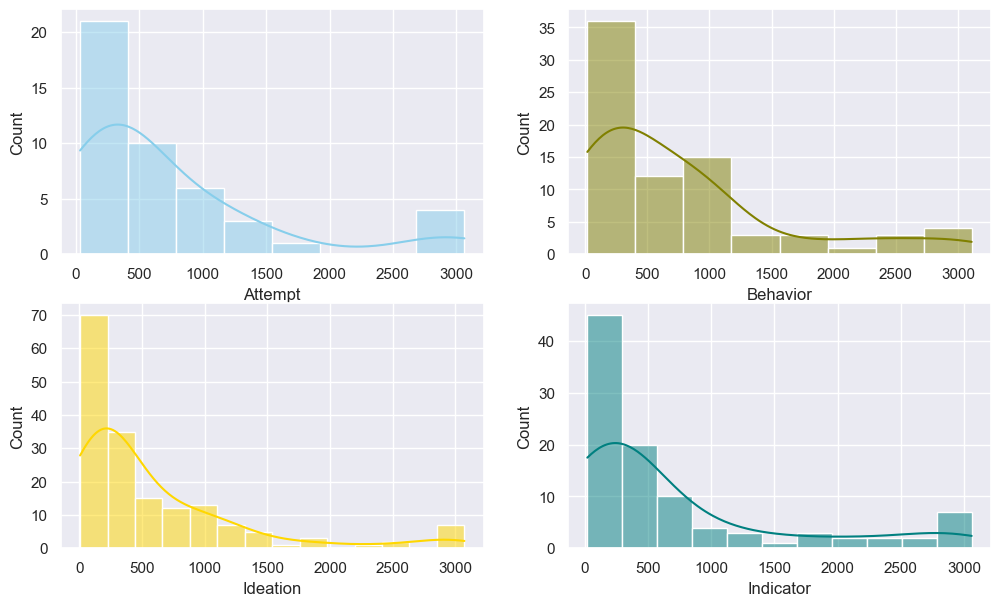
\includegraphics[width=\textwidth]{document_size_length_in_each_class.png}
\caption{Document size length in each class of suicidal category and samples frequency}
\label{reddit_cssrs_doc_len_freq}
\end{figure}
%
\subsubsection{Dataset Imbalance Handling}
From figure~\ref{reddit_cssrs_doc_len_freq} it is observed that number of samples in the attempt category is very low compared to other categories. To increase the dataset size balancing samples of each class, synthetic dataset is prepared. Text Data augmentation \cite{bayer2022survey} is applied.
Categorical features are mixed together shuffled and then grouped into fixed sized tokens. Random Shuffling is applied with various seed. It is considered as sample document for specific category. This process continues until we found desired number of samples. Then synthetic samples are combined with other samples to prepare train classifier dataset. 

\subsection{Testing/Validation Dataset} 
For testing dataset is collected from kaggle. It is an opesource dataset publicly available in kaggle collected from reddit website by a pushshift API contained suicide and depression category. The dataset contains posts of \enquote{SuicideWatch} and \enquote{depression} subreddits. \enquote{SuicideWatch} and \enquote{depression} posts were collected from roughly 2008 to 2021. The datasets comprised of 232,074 post annotated for binary classification as suicidal or non-suicidal Depression in \cite{aldhyani2022detecting} for detecting suicidal ideation. In this research trained classifier is applied to detect class on this two category. Main objective is to determine the suicide categories (indicator, ideation, behavior, attempt, supportive) within this dataset. 


\section{Methodology}\label{methodolo}
In this research supervised and unsupervised both type of data modeling is conducted. Unsupervised LDA modeling explores the key features, depict coherent terms related to specific suicide category. Supervised model is applied to train machine learning classifier to determine suicidal severity categories. Trained classifier, detects the suicidal risk within given post which contains depression post. Thereby analyzing result statistically suicidal tendency significance in depression post can be observed. This whole process is depicted in Figure \ref{fig:res_diagram}. Exploratory analysis started with dataset pre-processing. Most common techniques of NLP for data pre-processing is applied mentioned in the section \ref{data_preprocessing}. 

\subsection{Data Pre-processing}\label{data_preprocessing}
Social media dataset are Text data which needs data pre-processing, cleaning, feature extraction and data mining related NLP tasks.
\begin{enumerate}[label=(\roman*)]
\item Dataset noises such as: unnecessary quotes, special characters, punctuation etc and stop words are removed. Then further pre-processing is conducted which are followed for standard data cleaning process for NLP task. 
\item Morphological analysis is conducted to retrieve root words, process involves stemming, lemmatization etc.
\item Sentences are divided into equal-length fragments, and null word padding is applied to keep sample documents length same. Thereby corpus is prepared for further analysis.
\item Features are passed through a process in which features are converted to corresponding IDs and sentences which contain a series of IDs represented as vector. The embedding is another term that is frequently used in relation to vector text analysis. 
\end{enumerate}

From the pre-processed dataset tokenized corpus data is prepared. N-grams are generated (unigrams, Bi-grams, trigrams, etc.). To observe the most common n-grams. Word Clouds are prepared (\ref{redditdist_twitterdist_wordcloud}) where the size of each n-gram is proportional to its frequency identify patterns of co-occurring terms. 

\subsection{Latent Dirichlet Allocation (LDA)}
\label{lda_mdel}
LDA topic modeling \cite{jelodar_latent_2019, gupta_pan_lda_2021, pichardo_lagunas_svd_lda_2015, selvi_classification_2019} is used in this research scope that considers documents are mixed of topic based on distribution of words. The objective is to explore the hidden topic and the topic-word distributions, presumably describe the sample documents. An expression of the LDA model is described below:  
\begin{equation}
P(\theta_d,z,w\|\alpha,\beta)=P(\theta_d\|\alpha)\prod^N_{n=1}P(z_{d,n}\|\theta_d)P(w_{d,n}\|z_{d,n},\beta)
\end{equation}
Where $w_{d,n}$ the $n_{th}$ word in document $d$, $z_{d,n}$ the topic assigned to the $n_{th}$ word in document $d$, $\alpha,\beta$ are the Dirichlet LDA model parameters. controls per-document topic distribution, and per topic word distribution. $\theta_d$ represent the topic distribution. $P(\theta_d \| \alpha)$ Dirichlet 
distribution representing the document-topic distribution, $P(z_{d,n}\|\theta_d)$ is the word topic assignment for the $n_{th}$ word in document $d$, $P(w_{d,n}\|z_{d,n},\beta)$ is the distribution representing the observed word given a topic. 


Different techniques have been developed to perform topic modeling in the unsupervised topic modeling domain of Natural Language Processing (NLP), having their own strengths and limitations \cite{vayansky2020review, abdelrazek2022topic, yi2009comparative}. Apart from LDA, Mallet LDA, Structural Topic Model (STM), Hierarchical Dirichlet Process (HDP), Non-Negative Matrix Factorization (NMF), Latent Semantic Analysis (LSA) etc are also prevailing and can be considered for comparative research study.

\subsubsection{Topic models comparative analysis}
While some variations of LDA, Mallet LDA is considered for large corpus processing and analysis \cite{vayansky2020review, abdelrazek2022topic, Comparison_Topic_Modeling_Algorithms}. It focuses on scalability, If large corpus needs to analyze, Mallet LDA might be more suitable. LDA in general can still be efficiently applied to moderately sized corpora. Analyzing topics within the context of metadata, STM could be a better fit. Hierarchical Dirichlet Process (HDP) can be useful when we cannot guess the number of topics in advance. As a baseline model LDA is often considered one of the most prominent choices. In \cite{Comparison_Topic_Modeling_Algorithms} LSI, NMF and LDA are compared in terms of coherence and similarity measures for social media dataset and in their analysis LDA is observed most effective measures. In this study Reddit corpus LDA applied to determine dominant topics and explore correlations or co-occurrences. LDA off-the-selves python libraries produces interpretative results for exploratory topic analysis. The identified topics are represented as distributions over words, making it easy to assign meaningful labels to topics. Hence, LDA serves as a baseline for topic modeling in this research. However, how many topics are ideal it is needed to determine (see section \ref{coherence_equations}) that represents topic modeling quality.

\subsubsection{LDA model coherence}
\label{coherence_equations}
Coherence score estimates optimal number of topics. In this research scope coherence is measured to determine how coherent topic terms are \cite{mimno2011optimizing}. Using this score quality of the topics produced by LDA is assessed and ensures that the topics generated are statistically significant. Coherence \(C_{topic}\) can be expressed as follows  
\begin{equation}
C_{topic}=\sum^N_{i=1} \frac{1}{N(N-1)}\sum^i_{j=1} PMI(w_i,w_j)
\end{equation}
Where, \(PMI\left( w_{i},w_{j} \right)\) represent pointwise mutual information statistical association between two words occurring together. PMI score indicates that the two words are more closely related within a topic. \(PMI\left( w_{i},w_{j} \right)\) represents  
\begin{equation}
\(PMI\left( w_{i},w_{j} \right) = \log\frac{P\left( w_{i},w_{j} \right)}{P\left( w_{i} \right)P\left( w_{j} \right)}\)
\end{equation}
where \(P\left( w_{i},w_{j} \right)\) is joint probability of occurrence of words \(w_{i}\) and \(w_{j}\).  

\subsection{Supervised Modeling}
Various off-the-selves Machine learning and Deep Learning models are used for supervised classification of suicide and depression in several studies \cite{castillo2020suicide, chancellor2020methods, zhang2022natural}. 
There is conception that Deep learning models performs better than standard machine learning approaches. However, traditional machine learning models can outperform deep learning methods when extracted or filtered features are fitted into the training process. In this research cleaned features are feed into machine learning models for classification. 
\subsubsection{Classification}
In this research pre-processed dataset converted to vector using cutting edge vectorizers. Feature vector is feed into machine learning classifier which is trained to determine suicide intensity label in depression post. Various vectorization methods are present \cite{aldhyani2022detecting, wang2020depression, shetty2020predicting}. TF-IDF and Word2Vec vectorizers are applied here. Following approach is applied in this study for supervised classification
\begin{enumerate} [label=(\roman*)]
\item Pre-processed and useful features are used from Reddit's 500 post CSSR dataset for classifier Training
\item Used count vectorizer and TFIDF transformer to generate vectors for the dataset
\item Trained classifier to determine the categories of various suicidal intensities
\end{enumerate}
Research methodology is portrayed in figure~\ref{fig:res_diagram} 
\begin{figure}[h!]
\centering
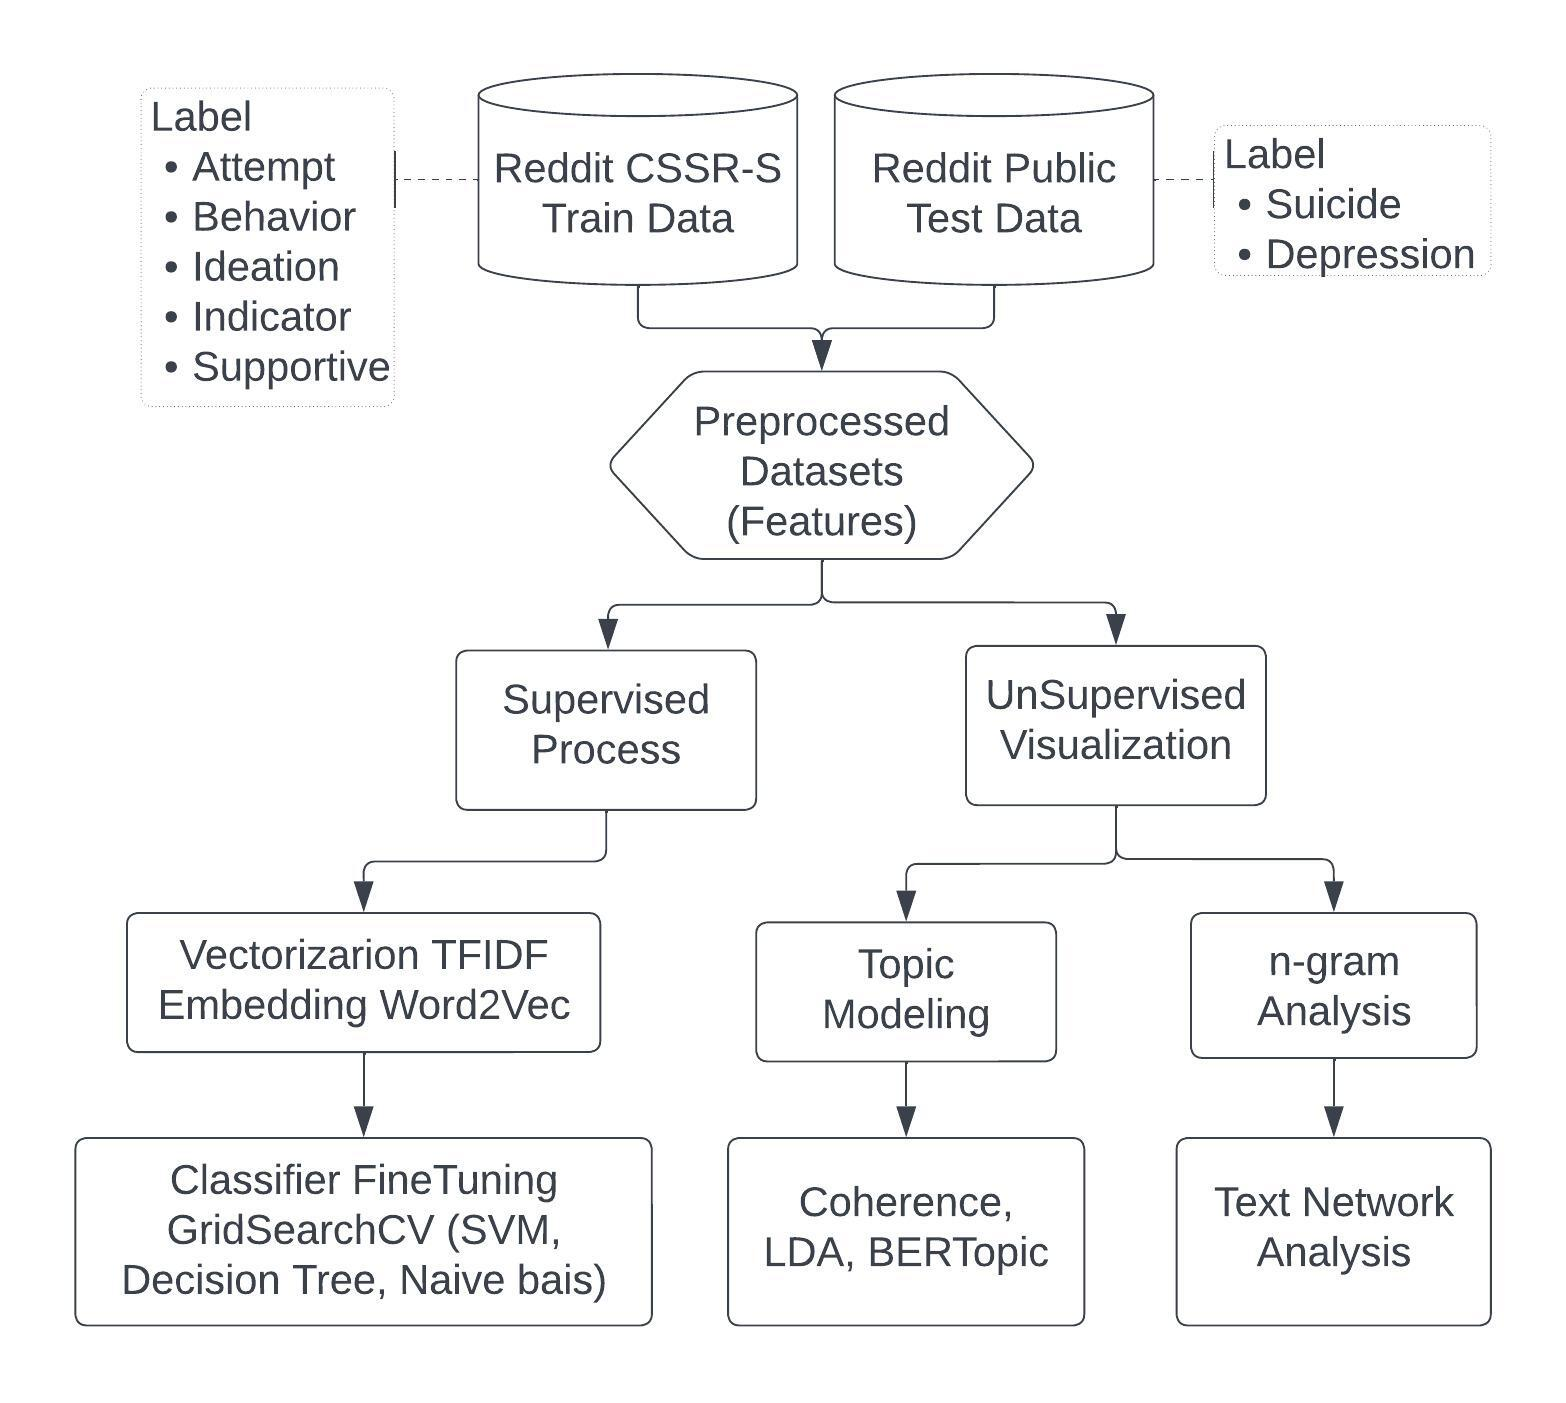
\includegraphics[width=0.8\textwidth]{res_diagram.jpeg}
\caption{Research Methodology overview}
\label{fig:res_diagram}
\end{figure}

\section{Exploratory analysis of features}
\label{exp_anal}
After pre-processing document samples contains only noise free features. Document length frequency and features distribution is depicted in Figure \ref{redditdist_twitterdist_together}. From the frequency distribution we can see some of the document sizes are very large. Hence, larger sentences are chopped and one sentence become multiple sentences of features keeping the label same. 
\begin{figure}[H]
\centering
\begin{subfigure}{0.45\textwidth}
    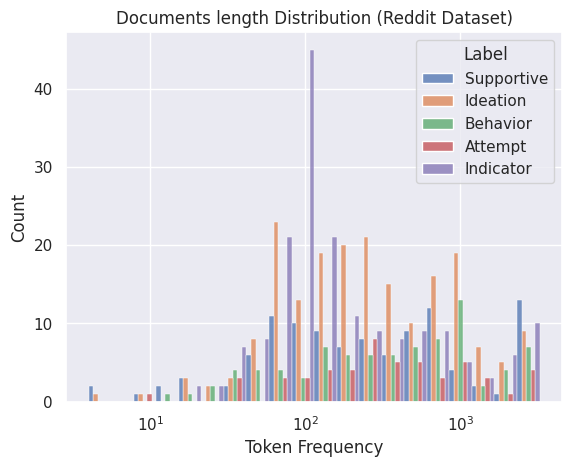
\includegraphics[width=\textwidth]{reddit_dist.png}
    \caption{Training dataset distribution}
    \label{redditdist}
\end{subfigure}
\hfill
\begin{subfigure}{0.45\textwidth}
    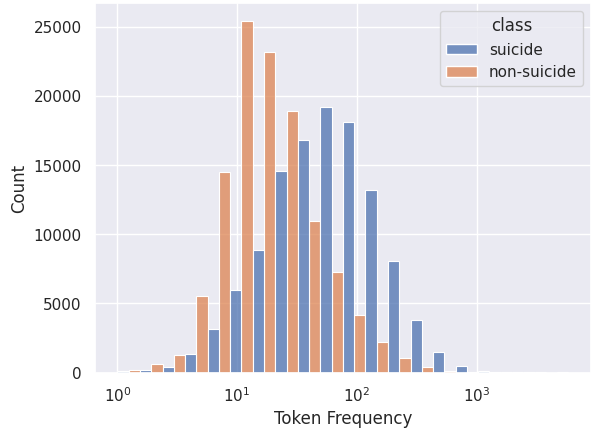
\includegraphics[width=\textwidth]{twitterdist.png}
    \caption{Testing dataset distribution}
    \label{twitterdist}
\end{subfigure}       
\caption{Train and Test dataset distribution}
\label{redditdist_twitterdist_together}
\end{figure}

\subsection{Training dataset exploration}
Uni-gram Word cloud is showed in figure \ref{redditdist_twitterdist_wordcloud} to depict each category and influence of dominant keywords based on frequency.  
\begin{figure}[h!]
\centering
\begin{subfigure}{0.45\textwidth}
    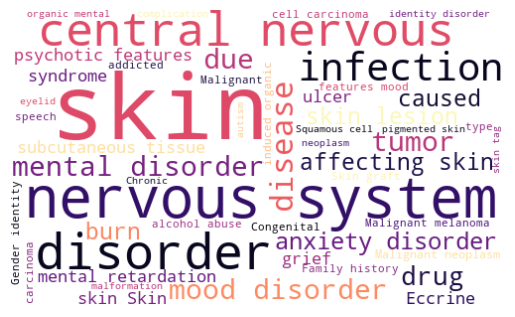
\includegraphics[width=\textwidth]{indicator_word_cloud.png}
    \caption{Indicator category word high impact words are anxiety, disease, disorder, nervous etc}
    \label{redditdist}
\end{subfigure}
\hfill
\begin{subfigure}{0.45\textwidth}
    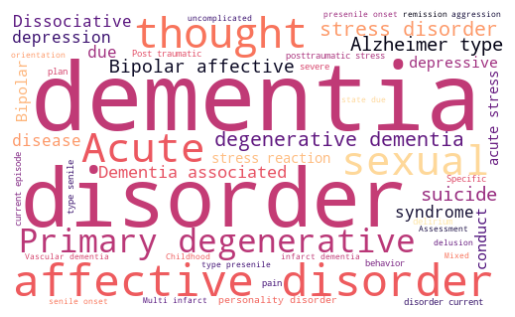
\includegraphics[width=\textwidth]{Ideation_word_cloud.png}
    \caption{Ideation category word cloud high impact words are dementia, affective disorder, stress, bipolar personality}
    \label{twitterdist}
\end{subfigure}      
\centering
\begin{subfigure}{0.45\textwidth}
    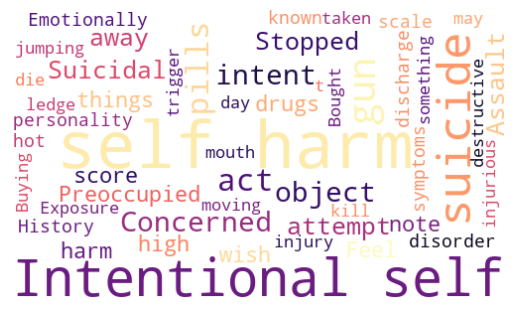
\includegraphics[width=\textwidth]{Behavior_word_cloud.png}
    \caption{Behavior category word cloud high impact words are self-harm, suicidal, intentional etc.}
    \label{redditdist}
\end{subfigure}
\hfill
\begin{subfigure}{0.45\textwidth}
    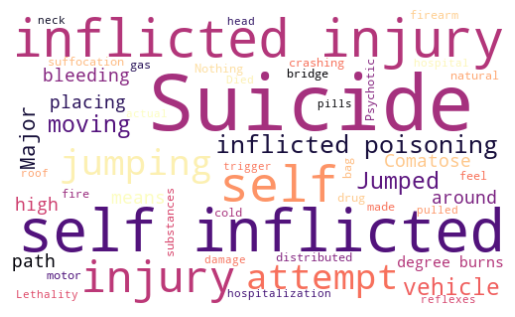
\includegraphics[width=\textwidth]{Attempt_word_cloud.png}
    \caption{Attempt category word cloud high impact keywords suicide, attempt, inflicted injury etc.}
    \label{twitterdist}
\end{subfigure}   
\caption{Train Reddit C-SSRS dataset word cloud distribution represents that there are overlapping features between Indicator with Ideation and Behavior with Attempt categories}
\label{redditdist_twitterdist_wordcloud}
\end{figure}
Visualizing the word cloud it is revealed there are correlation between Ideation and Indicator, Behavior and Attempt categories.  

\subsubsection{Coherence estimation for LDA model}
To calculate the coherence score gensim library provides range of options such as \(u_{mass},c_{v},c_{uci},c_{npmi}\). \(u_{mass}\) and \(c_{v}\)These two methods are most popular. For given topic with words \(\{ w_{1},w_{2},w_{3},\ldots..,w_{n}\}\) a fixed context window size is provided (default size 10 words) then coherence score is calculated using an equation \(\sum_{j = 1}^{i}{PMI}\left( w_{i},w_{j} \right)\) which provides negative coherence score. \(c_{v}\) can be expressed as  
\begin{equation}
\(c_{v} = \frac{1}{N(N - 1)}\sum_{j = 1}^{i}{similarity\left( w_{i},w_{j} \right)}\)
\end{equation}
in which \(similarity\left( w_{i},w_{j} \right)\) represent the pairwise similarity between terms based on \(PMI\left( w_{i},w_{j} \right)\) scores. \(c_{v}\) provides a positive coherence score. Higher coherence values (higher than 0.5) indicate that the topics are moderately coherent and representative of meaningful themes within the text data.

\begin{figure}[h!]
\centering
\begin{subfigure}{0.45\textwidth}
    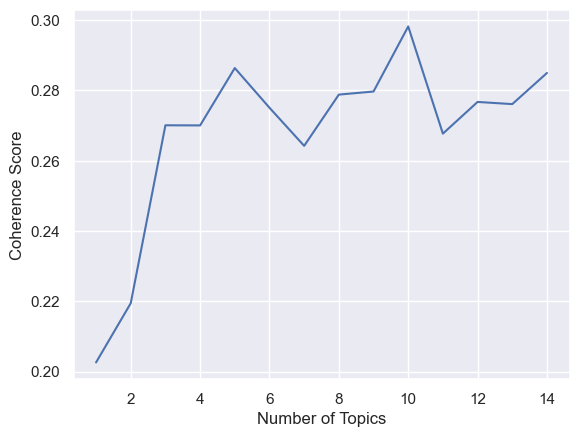
\includegraphics[width=\textwidth]{cv_indicator.png}
    \caption{Indicator category word cloud}
    \label{redditdist}
\end{subfigure}
\hfill
\begin{subfigure}{0.45\textwidth}
    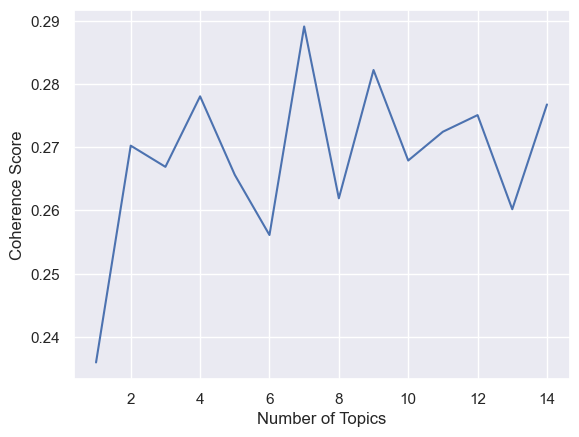
\includegraphics[width=\textwidth]{cv_ideation.png}
    \caption{Ideation category word cloud}
    \label{twitterdist}
\end{subfigure}      
\centering
\begin{subfigure}{0.45\textwidth}
    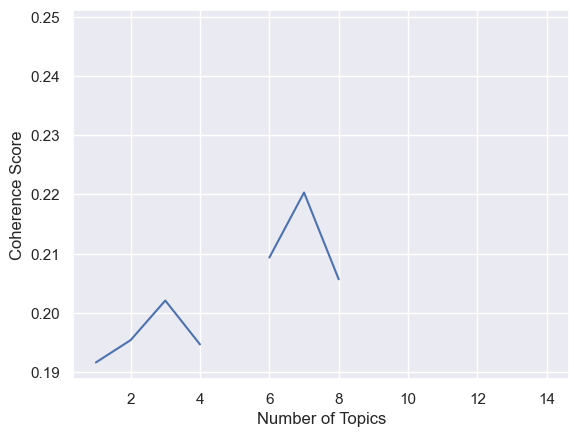
\includegraphics[width=\textwidth]{cv_behavior.png}
    \caption{Behavior category word cloud}
    \label{redditdist}
\end{subfigure}
\hfill
\begin{subfigure}{0.45\textwidth}
    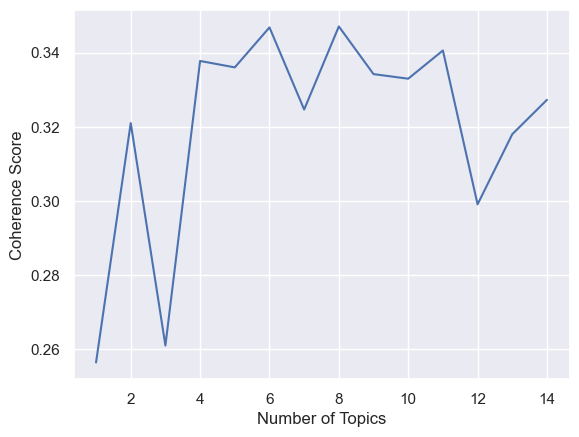
\includegraphics[width=\textwidth]{cv_attempt.png}
    \caption{Attempt category word cloud}
    \label{twitterdist}
\end{subfigure}   
%\caption{Train Reddit C-SSRS dataset word cloud distribution}
\label{redditdist_twitterdist}
\end{figure}


\subsubsection{Keywords importance visualization using LDA}
LDA driven results of various categories are visualized in this study to observe the latent topic using relative importance measurements depicted in figure \ref{indicator_weight_relative_imp}, \ref{ideation_weight_relative_imp}, \ref{behavior_weight_relative_imp}, and \ref{attempt_weight_relative_imp} and pyldvis library in figure~\ref{indicator_pyldvis}, \ref{Ideation_pyldvis}, \ref{Behavior_pyldvis} and \ref{Attempt_pyldvis}.
\begin{figure}[H]
    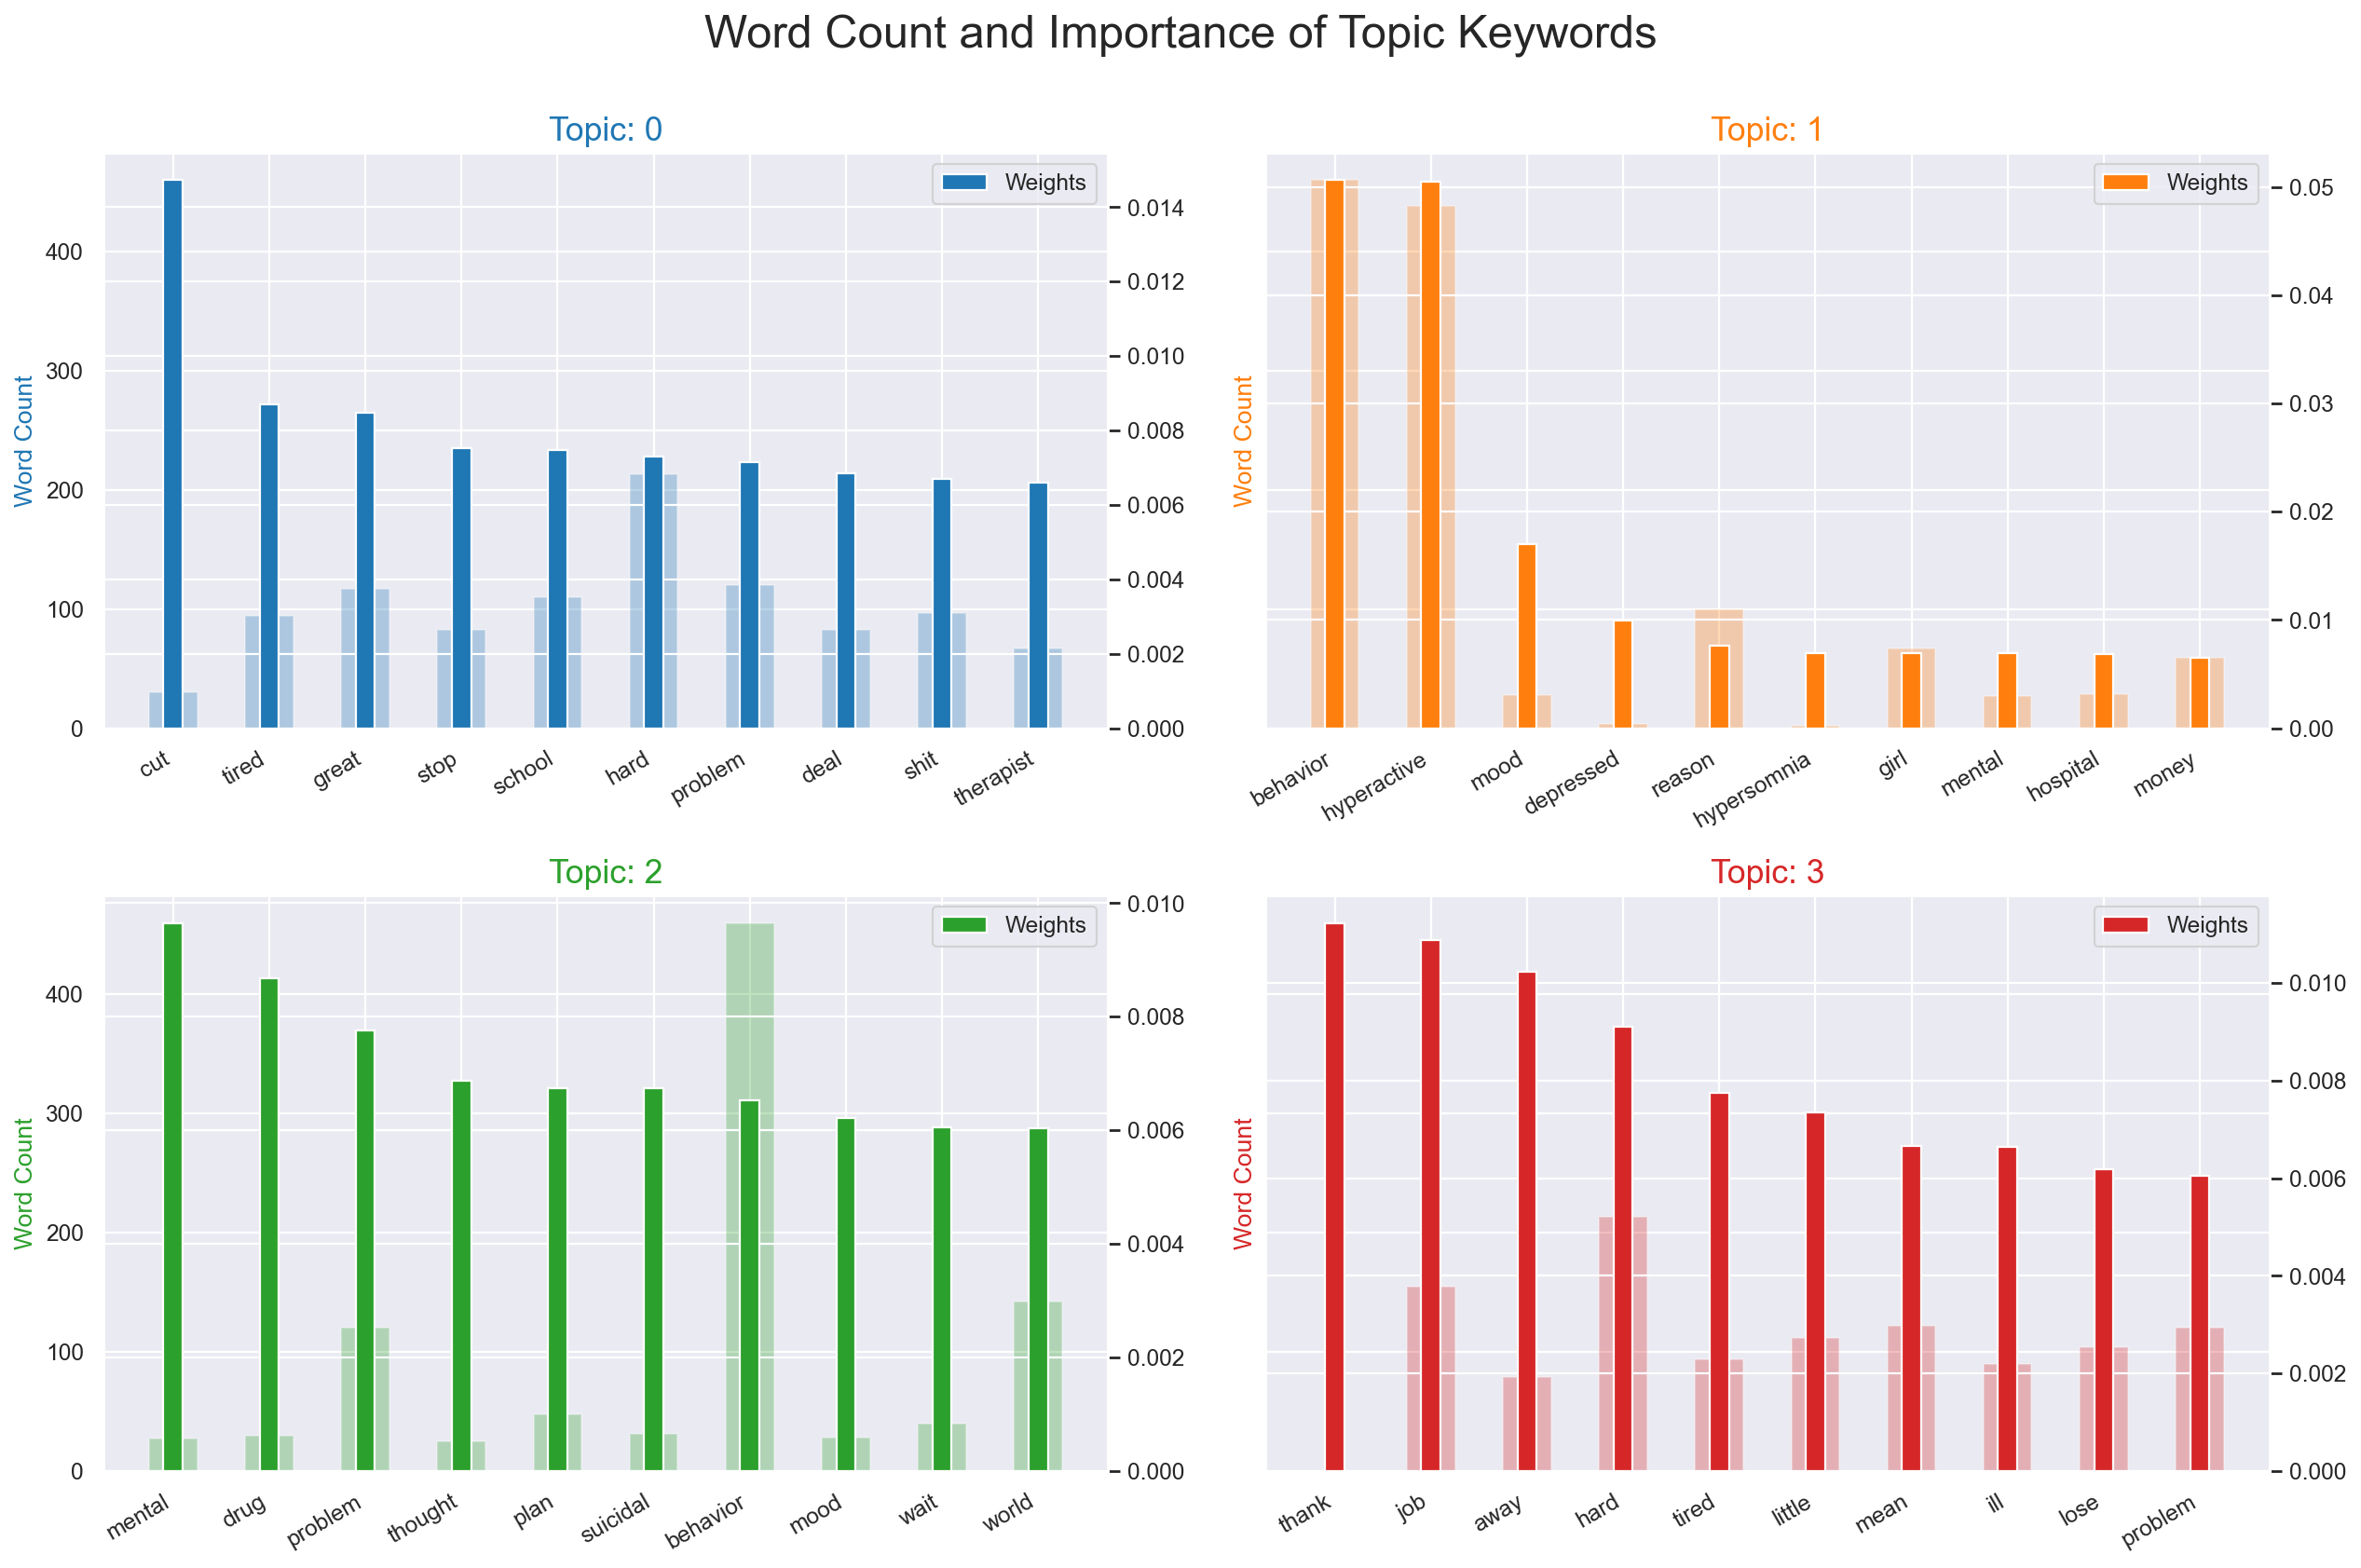
\includegraphics[width=\textwidth]{indicator_weight_relative_imp.png}
    \caption{Indicator category frequency vs LDA based relative Importance}
    \label{indicator_weight_relative_imp}
\end{figure}
\begin{figure}[H]
    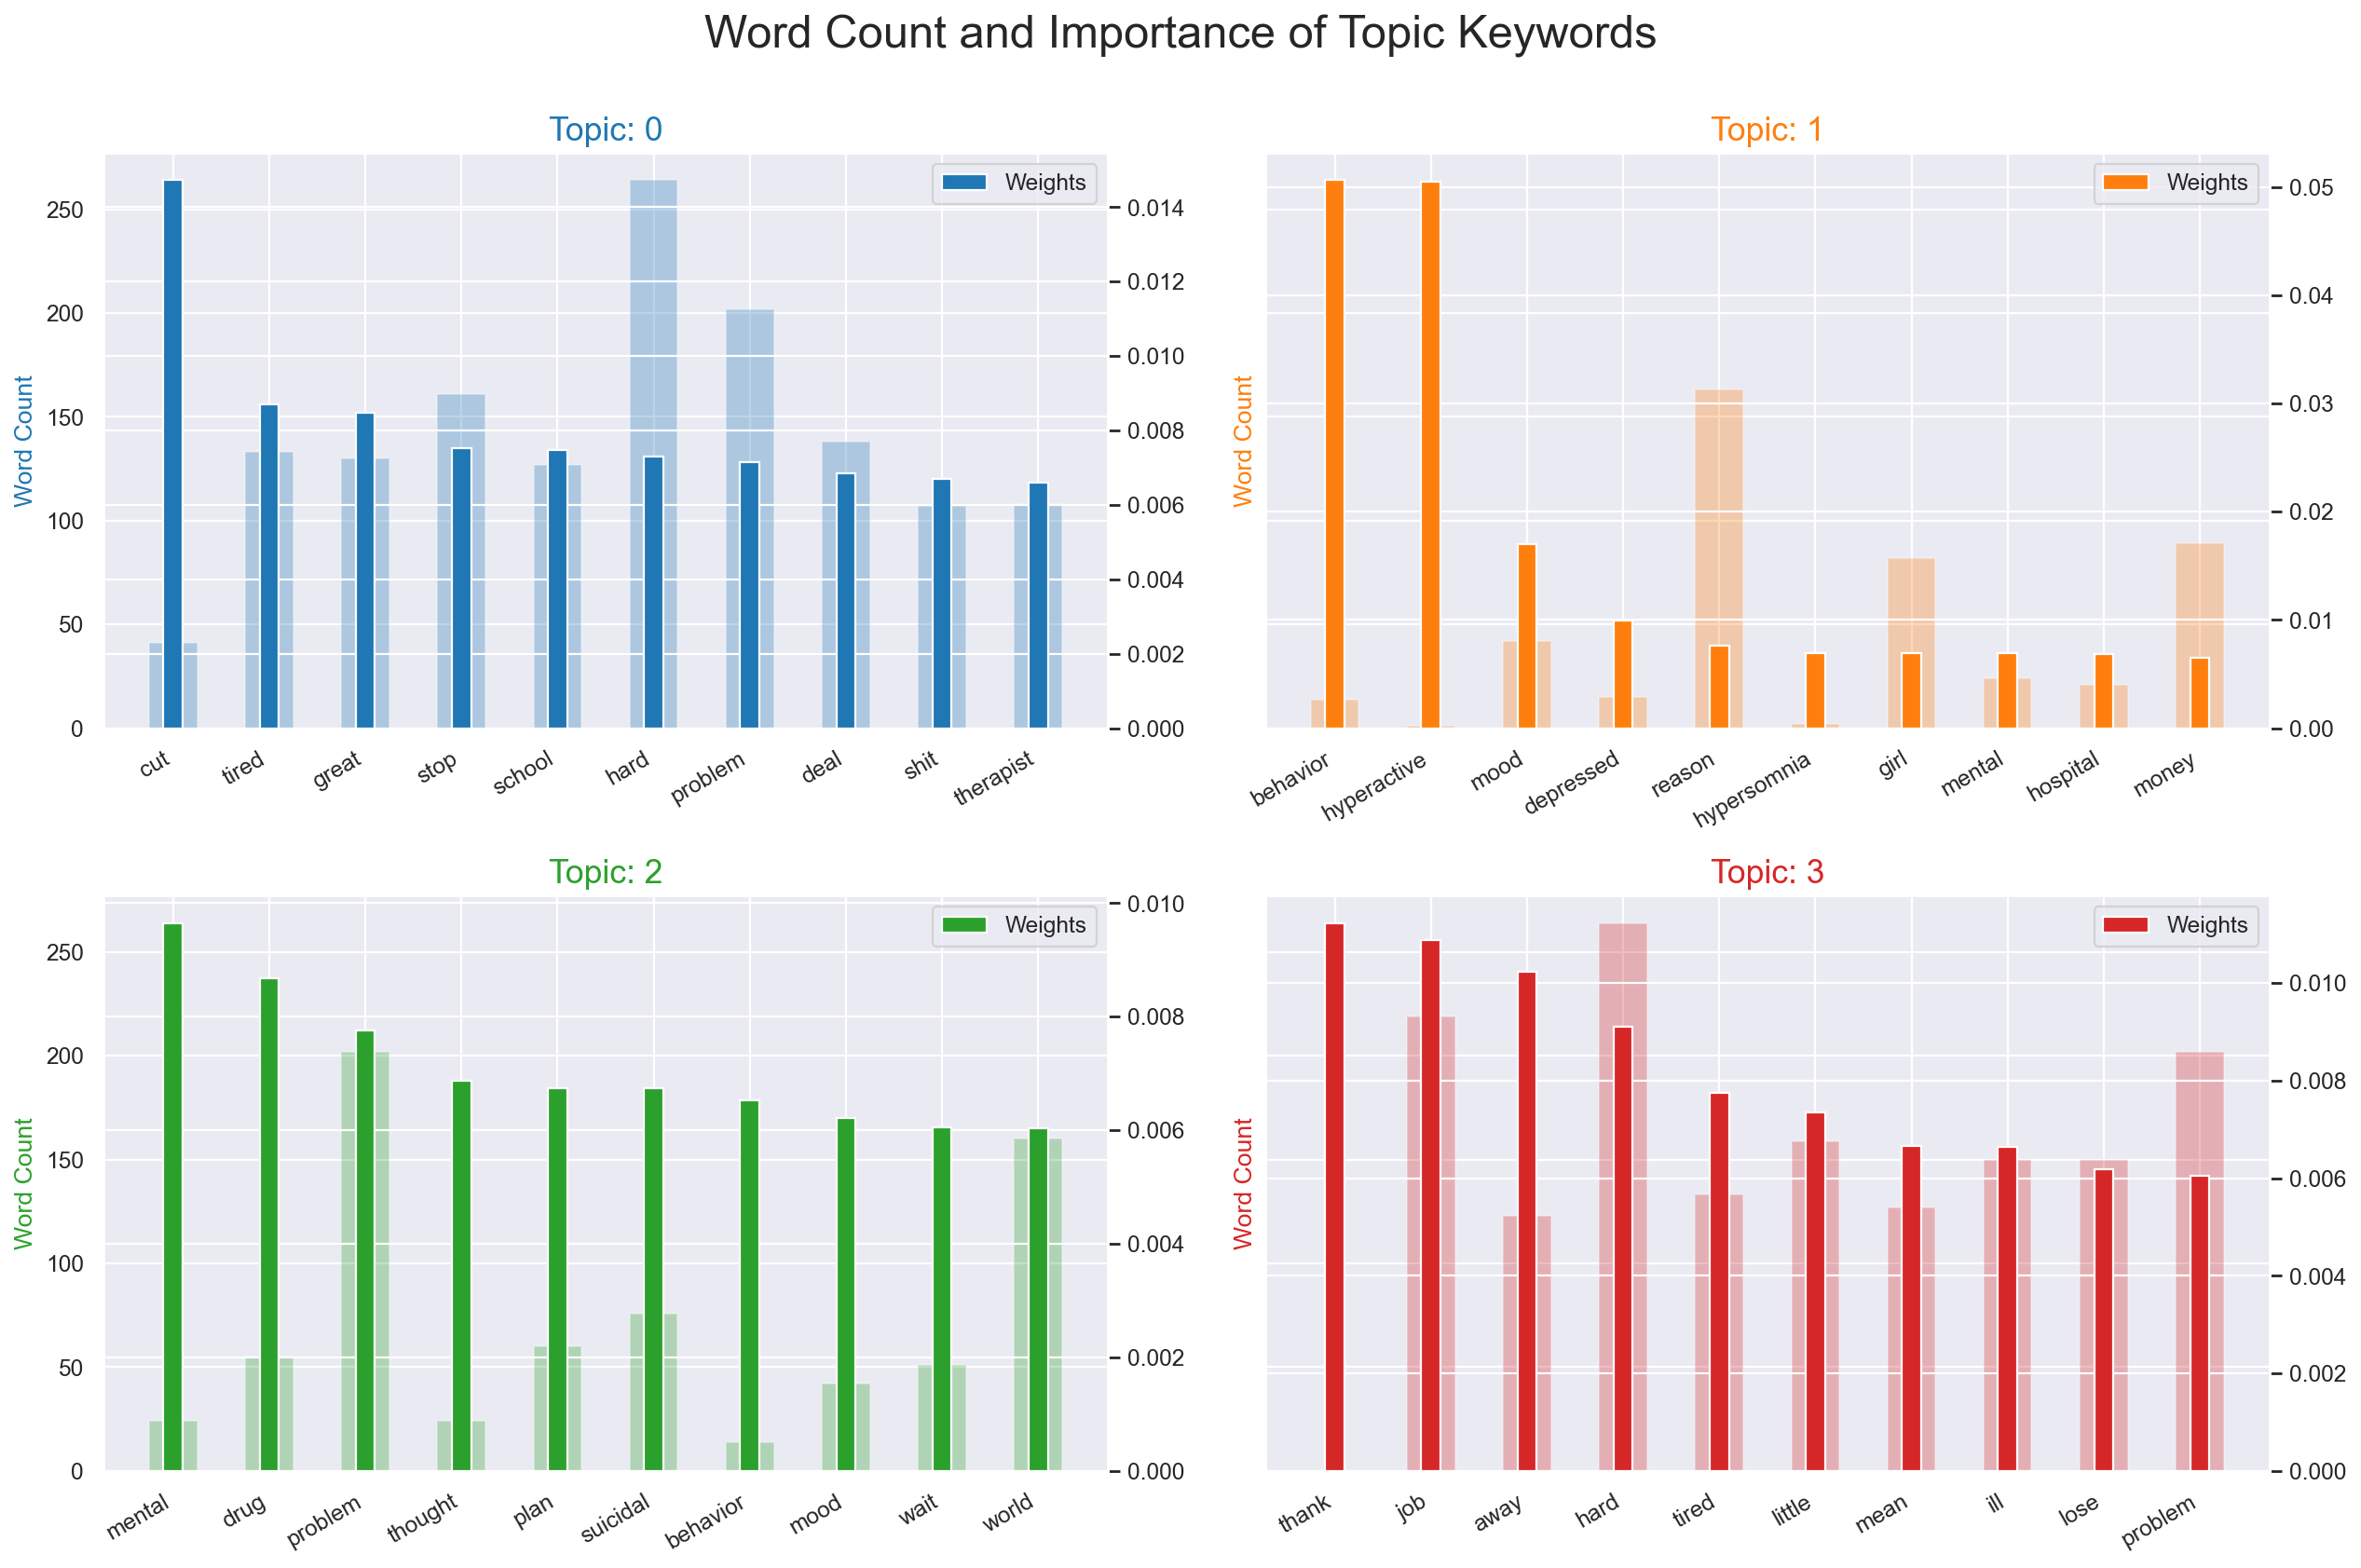
\includegraphics[width=\textwidth]{ideation_weight_relative_imp.png}
    \caption{Ideation category frequency vs LDA based relative Importance}
    \label{ideation_weight_relative_imp}
\end{figure}  
\begin{figure}[H]
    \includegraphics[width=\textwidth]{behavior_weight_relative_imp.png}
    \caption{Behavior category frequency vs LDA based relative Importance}
    \label{behavior_weight_relative_imp}
\end{figure}
\hfill
\begin{figure}[H]
    \includegraphics[width=\textwidth]{attempt_weight_relative_imp.png}
    \caption{Attempt category frequency vs LDA based relative Importance}
    \label{attempt_weight_relative_imp}
\end{figure}   


 

\begin{figure}[h!]
\centering
    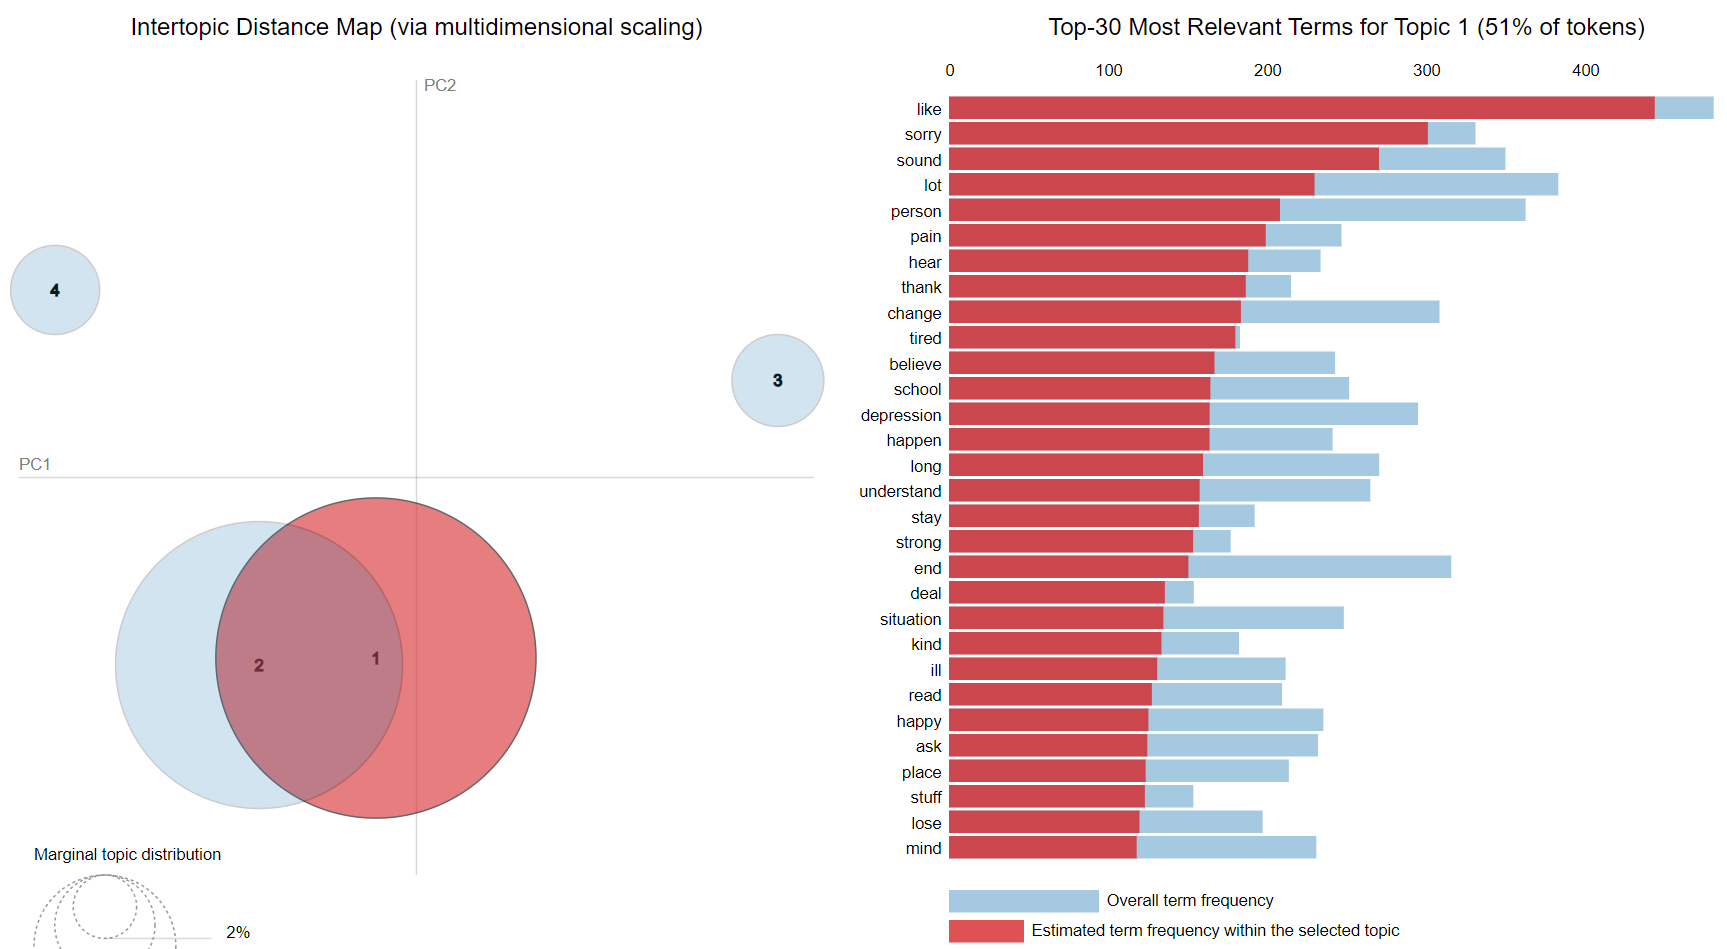
\includegraphics[width=\textwidth]{indicator_pyldvis.png}
    \caption{Indicator categories LDA's salient terms and topic visualization}
    \label{indicator_pyldvis}
\end{figure}

\begin{figure}[h!]
    \includegraphics[width=\textwidth]{Ideation_pyldvis.png}
    \caption{Ideation categories LDA's salient terms and topic visualization}
    \label{Ideation_pyldvis}
\end{figure}

\begin{figure}[h!]
    \includegraphics[width=\textwidth]{Behavior_pyldvis.png}
    \caption{Behavior categories LDA's salient terms and topic visualization}
    \label{Behavior_pyldvis}
\end{figure}

\begin{figure}[h!]
    \includegraphics[width=\textwidth]{Attempt_pyldvis.png}
    \caption{Attempt categories LDA's salient terms and topic visualization}
    \label{Attempt_pyldvis}
\end{figure}


\subsubsection{Combined topic modeling using BERTopic}
In this research scope BERTopic topic modeling applied which leverages deep learning pretrained BERT and c-TFIDF to create dense clusters of topics. Here BERTopic applied for the combined samples. Hence we can observe topics' distinctive feature characteristics, how distinctive indicator, Ideation, Behavior and Attempt categories features are.

\begin{figure}[h!]
\centering
\begin{subfigure}{0.45\textwidth}
    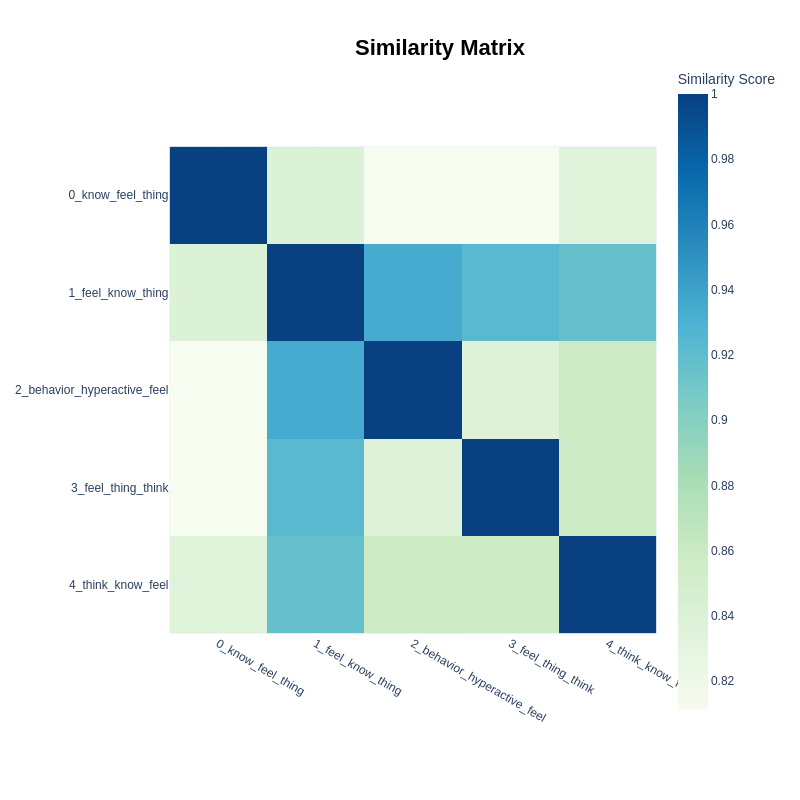
\includegraphics[width=\textwidth]{bertopic/combined_bertopic_topics_heatmap_frequency.png}
%    \caption{Ideation category word cloud}
    \label{redditdist}
\end{subfigure}
\hfill
\begin{subfigure}{0.45\textwidth}
    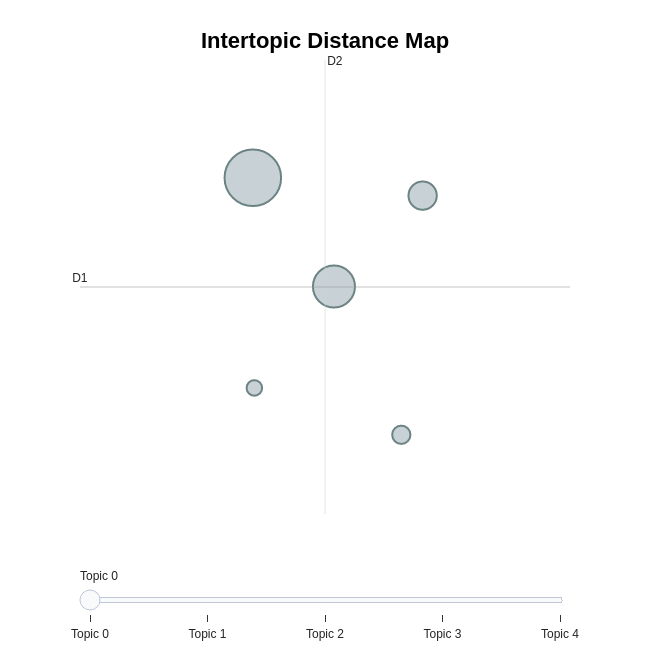
\includegraphics[width=\textwidth]{bertopic/combined_bertopic_topics_map_frequency.png}
%    \caption{Attempt category word cloud}
    \label{twitterdist}
\end{subfigure}   
\caption{Inter distance topic similarities}
\label{redditdist_twitterdist}
\end{figure}


\subsection{Test dataset exploration}
Frequency based comparison between two categories is conducted for depression and suicide for Test dataset in Figure \ref{dep_wordcloud_test} and \ref{sui_wordcloud_test} using Uni-gram based wordcloud. From this figure we can see that top ranked words those are occurring frequently tend to have slang and abusive terms compared to suicidal category. 
\begin{figure}[H]
\centering
\begin{subfigure}{0.45\textwidth}
    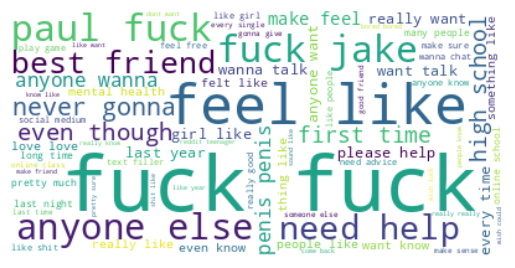
\includegraphics[width=\textwidth]{dep_wordcloud.png}
    \caption{Wordcloud in Depression category}
    \label{dep_wordcloud_test}
\end{subfigure}
\hfill
\begin{subfigure}{0.45\textwidth}
    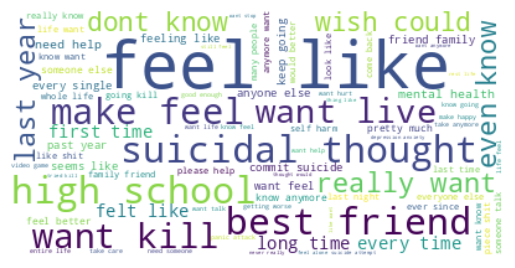
\includegraphics[width=\textwidth]{sui_wordcloud.png}
    \caption{Wordcloud in Suicide category}
    \label{sui_wordcloud_test}
\end{subfigure}
%\caption{Dataset features visualization and properties exploration}
%\label{features_vis_pro_exp}
\end{figure}

\subsubsection{Uni-gram Token distribution visualization}
In Test dataset samples a large number of documents are having low features. In figure~\ref{fig_Test_Dataset_token_frequency} the frequency of tokens in each class is depicted. Short sentence does not carry enough features which reveals does not carry enough information to be classified confidently by classifier algorithms. We started reducing the numbers of samples based on document length in Test dataset. By reducing the samples based on numbers of tokens present in a document (see Figure \ref{fig_Test_Dataset_token_frequency}). Documents length versus category frequency information is showed in this chart. This charts explains if we filter out the shorter comments suicide post become dominant class and depression post become outnumbered. 
%
\begin{figure}[H]
\centering
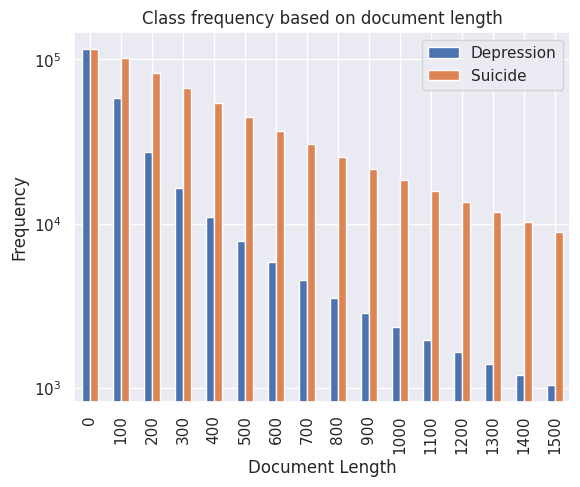
\includegraphics[height=6.5cm, width=0.7\textwidth]{doc_len.png}
\caption{Test Dataset token frequency in different Document Length}
\label{fig_Test_Dataset_token_frequency}
\end{figure}
%
The length of document and term frequency within the corpus is visualized in Figure \ref{redditdist_twitterdist}. From the distribution we can see that some of the document length are excessive long and contains more than 1000 tokens (within Train and Test both Dataset). Depression class document length are usually shorter in length. Depression document length are tend to be smaller than suicide document length. The difference showed an exponential pattern as length of document increases. Test dataset Reddit data distribution among depression and suicide class distribution ratio was equal. Filtering the class from figure \ref{fig_Test_Dataset_token_frequency} an interesting fact is revealed that depressed people does not want to comment very long. From figure~\ref{fig_Test_Dataset_token_frequency},  figure~\ref{dep_wordcloud_test} and \ref{sui_wordcloud_test} the following comments can be inferred
\begin{enumerate}
\item short statements likely to be more depression category
\item Depressive statements tend to have slang and abusive words
\item Suicidal thinking people’s post having very high frequency of “kill” “die” these type of words or phrases.
\item Rather suicidal depressed people want to share their thoughts with others using longer post.
\end{enumerate}

It is also interesting that there are many words have high frequency such as depression or depressed but belongs to suicide class. One important fact is revealed here is that we can see although suicide, suicidal these words has high frequency in Suicide class but depression, depressed also occurred in parallel with high frequency. However, it does not reveals any direct clues in terms of hypothetical relationships between the two category. It is difficult find pattern in which we can determine the depression and suicidal thought.  

\subsubsection{Bi-gram features relation exploration}
Bi-gram is analyzed for depression and suicide both categories. There are some Bi-grams which showed very high frequency. We called this special Bi-grams since. Special Bi-grams in the suicidal and depression both categories appeared highly frequent matter. Special Bi-grams are \enquote{mental health}, \enquote{feel like}, \enquote{make feel}, \enquote{high school}, \enquote{best friend}, \enquote{really want}, \enquote{suicide thought}, \enquote{friend family} showed high occurrences in the test dataset. Frequently occurred Bi-grams and its pattern in the corpus is explored. We want to analyze how these words have impact with its neighboring words depicted in Figure \ref{dep_chord} and \ref{suicide_chord}. To explore the impact of special bi-grams on the samples, special bi-gram terms containing samples are filtered from dataset. After that using lebel encoder Bi-grams are encoded as integers and then chord diagram is generated. We can observe meaningful relationship within the samples between the Bi-gram features.  


\begin{figure}[H]
\centering
    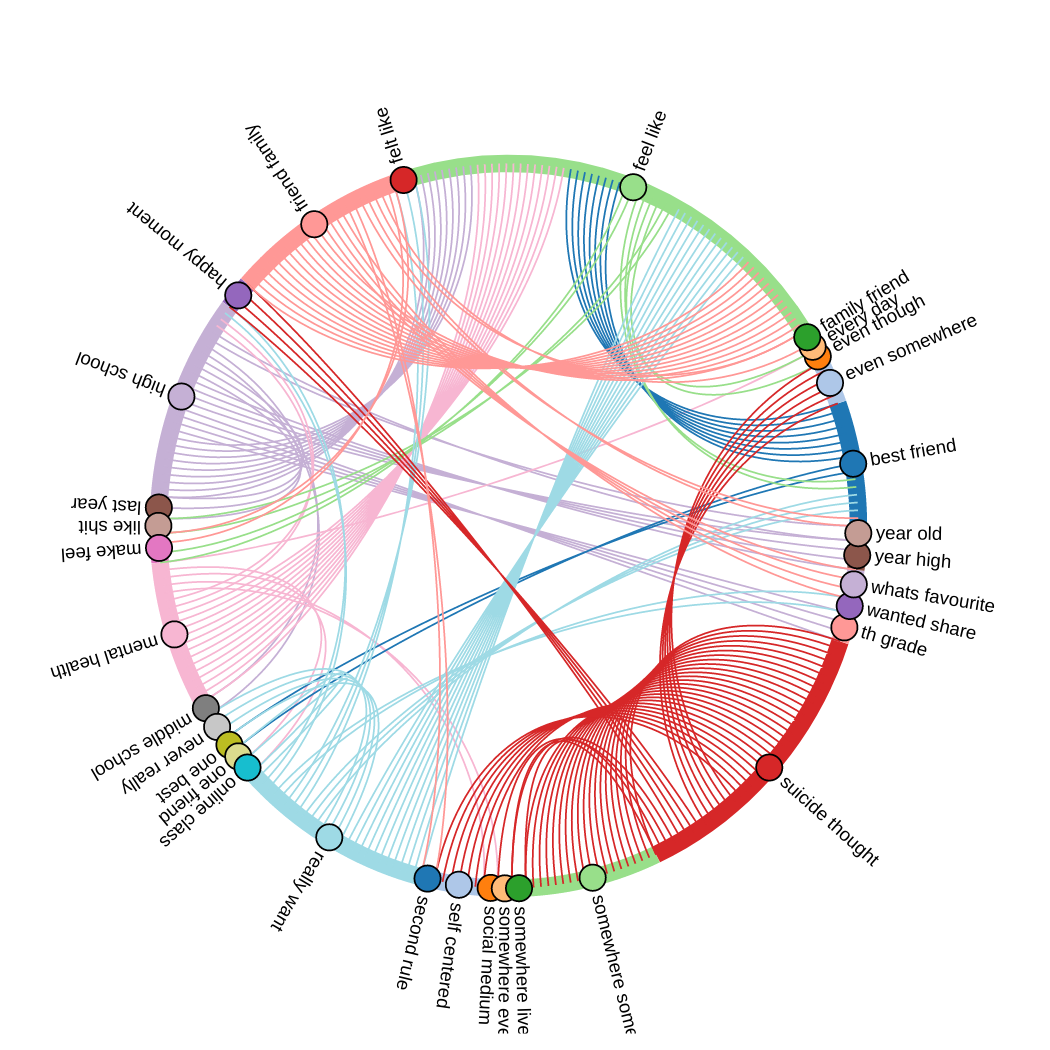
\includegraphics[width=0.75\textwidth]{dep_chord.png}
    \caption{Depression Chord diagram}
    \label{dep_chord}
\end{figure}

\begin{figure}[H]
\centering
    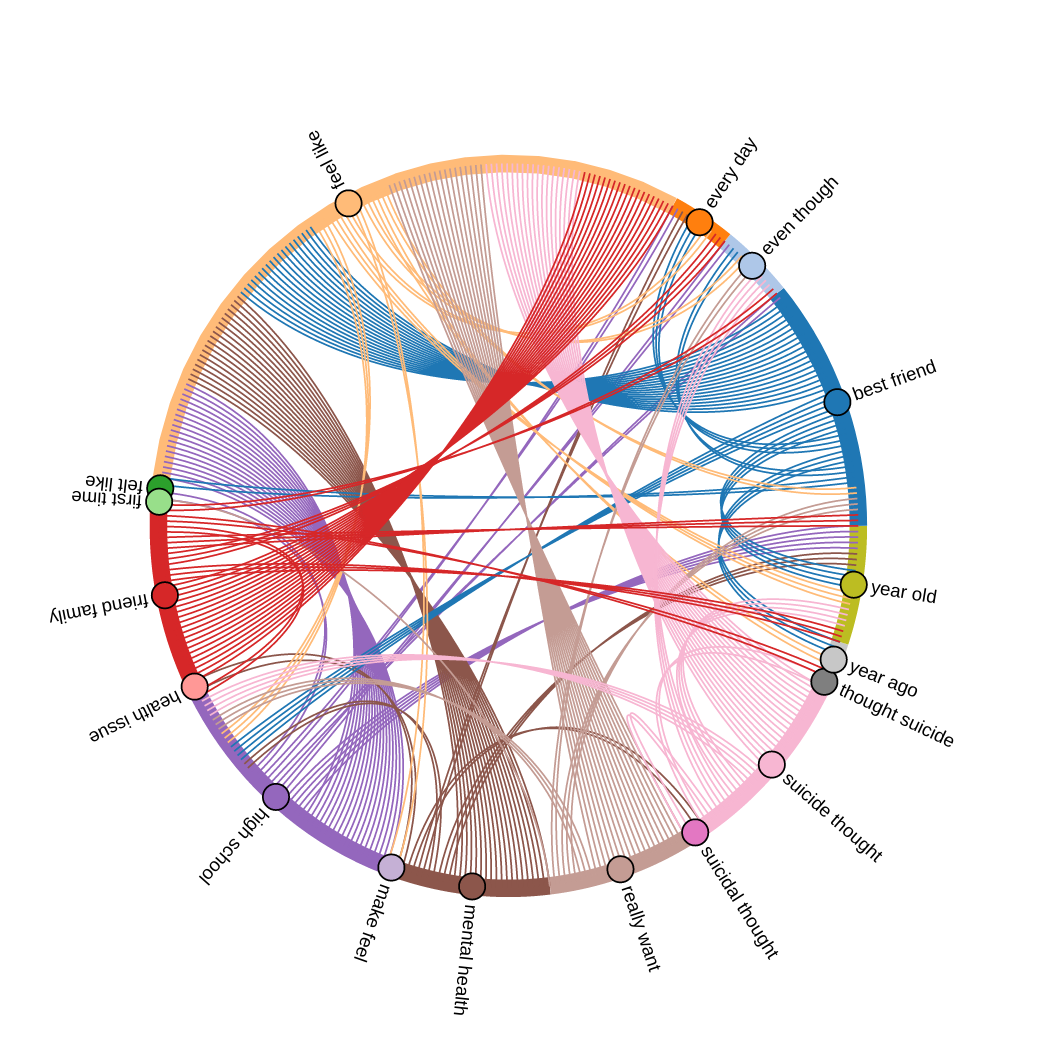
\includegraphics[width=0.75\textwidth]{suicide_chord.png}
    \caption{Depression Chord diagram}
    \label{suicide_chord}
\end{figure}        

From figure~\ref{dep_chord} and \ref{suicide_chord} two chord diagram interesting observation can be inferred (see Table \ref{chord_inference}). 
\begin{table}[h]
\begin{center}
\begin{flushleft}
\caption{Inference from chord diagrams}\label{chord_inference}%
\begin{tabular}{|l|p{6cm}|}
\toprule
\textbf{Depression} & \textbf{Suicide} \\
\midrule
self centered person is depressed & have mental health issue \\
having suicidal thought & share though with friends (high school friends, Best friends, family members) \\
want to go somewhere to live & having suicidal thoughts \\
spend happy moments & Friend family make feel better \\
\bottomrule
\end{tabular}
%\footnotetext{Inference from chord diagrams}
\end{flushleft}
\end{center}
\end{table}

Tri-grams or above did not reveals much meaning information, and therefore excluded for further experimental consideration. 


\section{Classification Results}
\label{classification_res}
How much depression can trigger suicidal thoughts is an interesting question. In this study classifier is trained on the suicidal intensity dataset. Then trained classifier is applied on the Depression/Suicide class dataset to investigate suicidal intensity in depression. Machine learning classification algorithms used for the experiments are mentioned in the Table \ref{Table_classification_alg}. The hyper-parameters settings for the classifiers are mostly sklearns' default settings. Classifiers are applied for the TFIDF vectorizer embedding (see results in figure~\ref{SVMTFIDF}) and also for Word2vec pretrained vectorizer model. Gridsearch technique of sklearn library is used in Two steps. From the selected classifiers to determine the best classifiers default parameters are applied and SVM showed most promising results. Then, to achieve highest accuracy hyper-parameters are feed into grid search. Using various set of parameters, from the experiments results we found almost 60\% accuracy for SVM model. From various set of values gridsearch for SVM SVC we found degree=2, gamma=0.7, kernel=rbf showed the highest accuracy. 
%
\begin{table}[h]
\begin{center}
\begin{flushleft}
\caption{Applied Machine Learning Classifiers and Parameters}\label{Table_classification_alg}%
\begin{tabular}{|l|p{8cm}|}
\toprule
\textbf{Classifiers} & \textbf{Hyper-Parameters [Some Specified and rest are default sklearn params]} \\
\midrule
K Nearest Neighbors & neighbors=5,  weights=\enquote{uniform} \\
SVM (SVC, Linear, SGD)& C=$0.1\sim 1.0$, kernel=\enquote{rbf/Linear/poly}, degree=$1\sim 3$\\
Gaussian Process Regressor & $\alpha$=$1^{-10}$ \\
Decision Tree & criterion=gini, splitter=\enquote{best}, min split=2  \\
Random Forest Ensemble & estimators=100, criterion=\enquote{gini}, min split=2, min leaf=1, max features=\enquote{sqrt}\\
Multi-layer perceptron & solver=\enquote{Adam}, $\alpha$=1, hidden layer=15 \\
AdaBoost Ensemble & estimators=50, learning rate=1.0, boosting algorithm=\enquote{SAMME.R}\\
Naive Bayes (GaussianNB) & smoothing=$1^{-9}$\\
\bottomrule
\end{tabular}
%\footnotetext{Inference from chord diagrams}
\end{flushleft}
\end{center}
\end{table}

%\begin{table}[h!]
%\begin{center}
%\begin{minipage}{174pt}
%\caption{Classifiers accuracy of models}\label{tab1}%
%\begin{tabular}{@{}lllll@{}}
%\toprule
%Classifier & Precision & Recall & Accuracy & F1 \\
%\midrule
%Nearest Neighbors & 0.926 & 0.924 & 92.3896 & 0.924\\
%RBF SVM & 0.942 & 0.924 & 92.3896 & 0.927\\
%Decision Tree & 0.901 & 0.848 & 84.7793 & 0.856\\
%Random Forest & 0.513 & 0.282 & 28.1583 & 0.167\\
%Neural Net & 0.942 & 0.927 & 92.6941 & 0.929\\
%AdaBoost & 0.905 & 0.898 & 89.8021 & 0.899\\
%Gaussian Process & 0.940 & 0.921 & 92.0852 & 0.924\\
%Naive Bayes & 0.923 & 0.918 & 91.7808 & 0.919\\
%QDA & 0.931 & 0.909 & 90.8676 & 0.912\\
%\botrule
%\end{tabular}
%\footnotetext{}
%\end{minipage}
%\end{center}
%\end{table}


\subsubsection{Suicidal Intensities visualization}
From the results we can see that suicidal ideation between depression and suicidal categories number of samples are very similar (figure~\ref{Suicidal_int_vis}). Within depression more number of samples are showed suicidal indicator category compared to suicide which is an interesting result. Suicidal behavior and attempt is comparatively high within the suicidal category than depression. Hence, figure~\ref{SVMTFIDF} result seems to be pretty obvious, except for suicidal ideation category. Also for the suicidal indicator symptoms are higher within the depression category. 

\begin{figure}[H]
\centering
\begin{subfigure}{0.45\textwidth}
    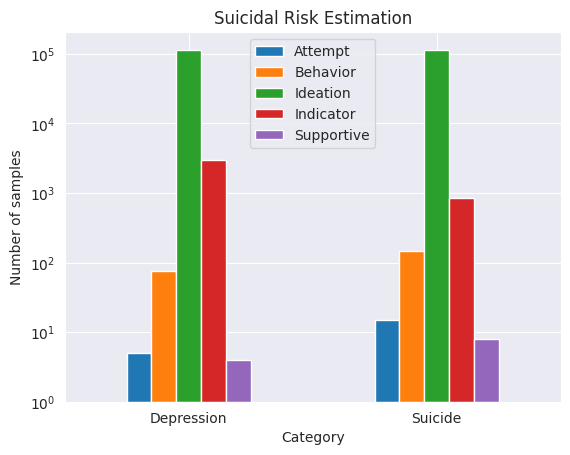
\includegraphics[width=\textwidth]{grid_svm.png}
    \caption{SVM classifier applied for TFIDF vectorizer}
    \label{SVMTFIDF}
\end{subfigure}
\hfill
\begin{subfigure}{0.45\textwidth}
    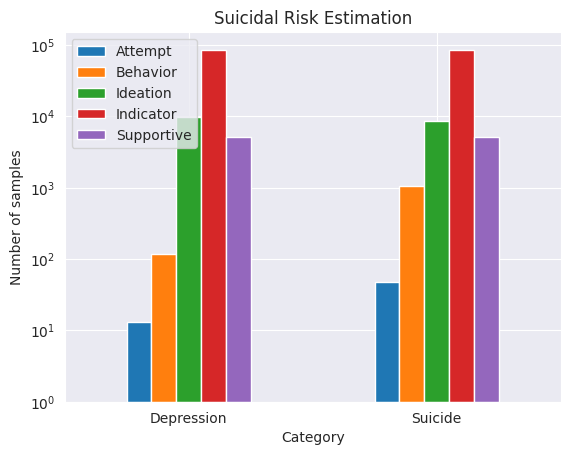
\includegraphics[width=\textwidth]{glove_vec.png}
    \caption{SVM classifier applied for Glove Word2Vec Pretrained model vectorizer}
    \label{GloveWord2Vec}
\end{subfigure}        
\caption{Visualizing suicide intensities within Depression/Suicide class}
\label{Suicidal_int_vis} 
\end{figure}
%z
For the word2vec vector embedding scenario supportive and indicator categories results are almost similar in depression or suicide both classes. There is slight difference is shown for suicidal ideation and within suicide class, suicidal ideation is slight higher. Except the behavior and attempt category for the rest categories depression and suicide showed almost similar number of samples. 

%\begin{figure}[H]
%\centering
%\begin{subfigure}{0.45\textwidth}
%    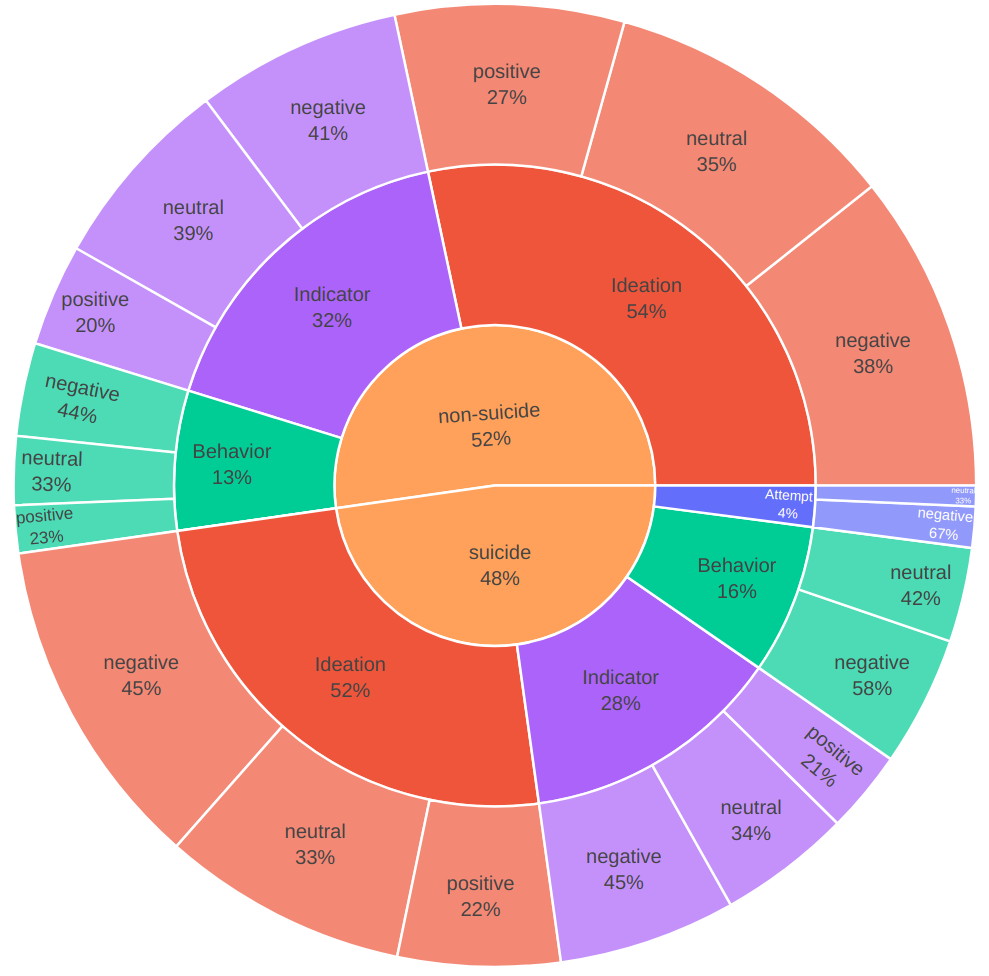
\includegraphics[width=\textwidth]{sentiment_sunburst.png}
%    \caption{First subfigure.}
%    \label{fig:first_sentiment_sunburst}
%\end{subfigure}
%\hfill
%\begin{subfigure}{0.45\textwidth}
%    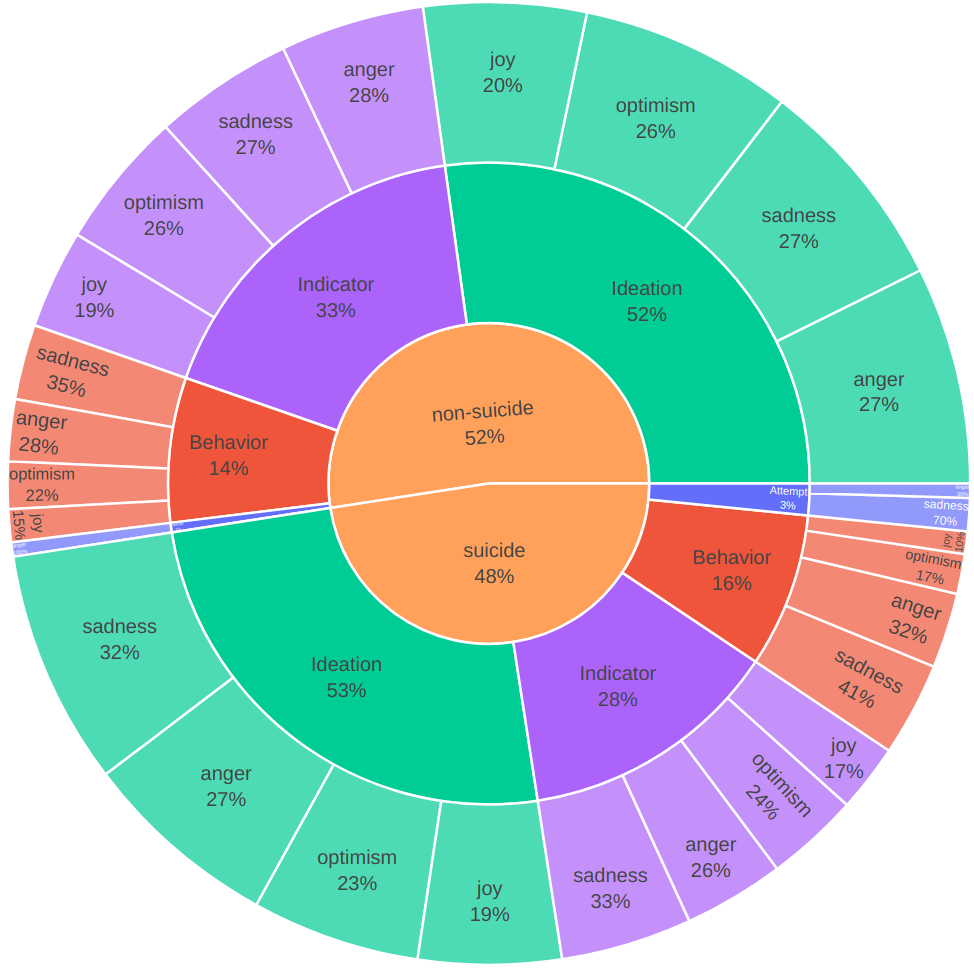
\includegraphics[width=\textwidth]{emotion_sunburst.png}
%    \caption{Second subfigure.}
%    \label{fig:second_emotion_sunburst}
%\end{subfigure}
%        
%\caption{Subreferences in \LaTeX.}
%%\label{fig:figures}
%\end{figure}
\section{Conclusion} 
\label{conclu}
Suicidal risk estimation task and classification samples to determine suicidal risk within social websites and blogs, techniques are discussed before. It is difficult to determine exactly since depression and suicide categorical variables are independent factor. The underlying correlation is difficult to formulate. However, to what extent depression level posses suicidal risk is not yet discussed before which is addressed in this study. This research explores various suicidal intensities in Reddit social media's depression post. Suicidal behavior and attempt showed higher number of samples within the suicide category compared to depression category. All these results seems logical and validates our experimental outcomes. Specially suicidal ideation, indicator showed similar patterns, expressing that depressed persons' comments has suicidal ideation and suicidal indicating symptoms. Results are susceptible to chosen classifier, chosen dataset, pretrained models vectors or embedding provided to the classifier. 

%\section{This is an example for first level head---section head}\label{sec3}
%
%\subsection{This is an example for second level head---subsection head}\label{subsec2}
%
%\subsubsection{This is an example for third level head---subsubsection head}\label{subsubsec2}
%
%Sample body text. Sample body text. Sample body text. Sample body text. Sample body text. Sample body text. Sample body text. Sample body text. 
%
%\section{Equations}\label{sec4}
%
%Equations in \LaTeX\ can either be inline or on-a-line by itself (``display equations''). For
%inline equations use the \verb+$...$+ commands. E.g.: The equation
%$H\psi = E \psi$ is written via the command \verb+$H \psi = E \psi$+.
%
%For display equations (with auto generated equation numbers)
%one can use the equation or align environments:
%\begin{equation}
%\|\tilde{X}(k)\|^2 \leq\frac{\sum\limits_{i=1}^{p}\left\|\tilde{Y}_i(k)\right\|^2+\sum\limits_{j=1}^{q}\left\|\tilde{Z}_j(k)\right\|^2 }{p+q}.\label{eq1}
%\end{equation}
%where,
%\begin{align}
%D_\mu &=  \partial_\mu - ig \frac{\lambda^a}{2} A^a_\mu \nonumber \\
%F^a_{\mu\nu} &= \partial_\mu A^a_\nu - \partial_\nu A^a_\mu + g f^{abc} A^b_\mu A^a_\nu \label{eq2}
%\end{align}
%Notice the use of \verb+\nonumber+ in the align environment at the end
%of each line, except the last, so as not to produce equation numbers on
%lines where no equation numbers are required. The \verb+\label{}+ command
%should only be used at the last line of an align environment where
%\verb+\nonumber+ is not used.
%\begin{equation}
%Y_\infty = \left( \frac{m}{\textrm{GeV}} \right)^{-3}
%    \left[ 1 + \frac{3 \ln(m/\textrm{GeV})}{15}
%    + \frac{\ln(c_2/5)}{15} \right]
%\end{equation}
%The class file also supports the use of \verb+\mathbb{}+, \verb+\mathscr{}+ and
%\verb+\mathcal{}+ commands. As such \verb+\mathbb{R}+, \verb+\mathscr{R}+
%and \verb+\mathcal{R}+ produces $\mathbb{R}$, $\mathscr{R}$ and $\mathcal{R}$
%respectively (refer Subsubsection~\ref{subsubsec2}).
%
%\section{Tables}\label{sec5}
%
%Tables can be inserted via the normal table and tabular environment. To put
%footnotes inside tables you should use \verb+\footnotetext[]{...}+ tag.
%The footnote appears just below the table itself (refer Tables~\ref{tab1} and \ref{tab2}). 
%For the corresponding footnotemark use \verb+\footnotemark[...]+
%


\noindent
The input format for the above table is as follows:



%%=============================================%%
%% For presentation purpose, we have included  %%
%% \bigskip command. please ignore this.       %%
%%=============================================%%

%%=============================================%%
%%% For presentation purpose, we have included  %%
%%% \bigskip command. please ignore this.       %%
%%%=============================================%%
%
%\begin{table}[h]
%\begin{center}
%\begin{minipage}{\textwidth}
%\caption{Example of a lengthy table which is set to full textwidth}\label{tab2}
%\begin{tabular*}{\textwidth}{@{\extracolsep{\fill}}lcccccc@{\extracolsep{\fill}}}
%\toprule%
%& \multicolumn{3}{@{}c@{}}{Element 1\footnotemark[1]} & \multicolumn{3}{@{}c@{}}{Element 2\footnotemark[2]} \\\cmidrule{2-4}\cmidrule{5-7}%
%Project & Energy & $\sigma_{calc}$ & $\sigma_{expt}$ & Energy & $\sigma_{calc}$ & $\sigma_{expt}$ \\
%\midrule
%Element 3  & 990 A & 1168 & $1547\pm12$ & 780 A & 1166 & $1239\pm100$\\
%Element 4  & 500 A & 961  & $922\pm10$  & 900 A & 1268 & $1092\pm40$\\
%\botrule
%\end{tabular*}
%\footnotetext{Note: This is an example of table footnote. This is an example of table footnote this is an example of table footnote this is an example of~table footnote this is an example of table footnote.}
%\footnotetext[1]{Example for a first table footnote.}
%\footnotetext[2]{Example for a second table footnote.}
%\end{minipage}
%\end{center}
%\end{table}
%
%In case of double column layout, tables which do not fit in single column width should be set to full text width. For this, you need to use \verb+\begin{table*}+ \verb+...+ \verb+\end{table*}+ instead of \verb+\begin{table}+ \verb+...+ \verb+\end{table}+ environment. Lengthy tables which do not fit in textwidth should be set as rotated table. For this, you need to use \verb+\begin{sidewaystable}+ \verb+...+ \verb+\end{sidewaystable}+ instead of \verb+\begin{table*}+ \verb+...+ \verb+\end{table*}+ environment. This environment puts tables rotated to single column width. For tables rotated to double column width, use \verb+\begin{sidewaystable*}+ \verb+...+ \verb+\end{sidewaystable*}+.
%
%\begin{sidewaystable}
%\sidewaystablefn%
%\begin{center}
%\begin{minipage}{\textheight}
%\caption{Tables which are too long to fit, should be written using the ``sidewaystable'' environment as shown here}\label{tab3}
%\begin{tabular*}{\textheight}{@{\extracolsep{\fill}}lcccccc@{\extracolsep{\fill}}}
%\toprule%
%& \multicolumn{3}{@{}c@{}}{Element 1\footnotemark[1]}& \multicolumn{3}{@{}c@{}}{Element\footnotemark[2]} \\\cmidrule{2-4}\cmidrule{5-7}%
%Projectile & Energy	& $\sigma_{calc}$ & $\sigma_{expt}$ & Energy & $\sigma_{calc}$ & $\sigma_{expt}$ \\
%\midrule
%Element 3 & 990 A & 1168 & $1547\pm12$ & 780 A & 1166 & $1239\pm100$ \\
%Element 4 & 500 A & 961  & $922\pm10$  & 900 A & 1268 & $1092\pm40$ \\
%Element 5 & 990 A & 1168 & $1547\pm12$ & 780 A & 1166 & $1239\pm100$ \\
%Element 6 & 500 A & 961  & $922\pm10$  & 900 A & 1268 & $1092\pm40$ \\
%\botrule
%\end{tabular*}
%\footnotetext{Note: This is an example of table footnote this is an example of table footnote this is an example of table footnote this is an example of~table footnote this is an example of table footnote.}
%\footnotetext[1]{This is an example of table footnote.}
%\end{minipage}
%\end{center}
%\end{sidewaystable}
%
%\section{Figures}\label{sec6}
%
%As per the \LaTeX\ standards you need to use eps images for \LaTeX\ compilation and \verb+pdf/jpg/png+ images for \verb+PDFLaTeX+ compilation. This is one of the major difference between \LaTeX\ and \verb+PDFLaTeX+. Each image should be from a single input .eps/vector image file. Avoid using subfigures. The command for inserting images for \LaTeX\ and \verb+PDFLaTeX+ can be generalized. The package used to insert images in \verb+LaTeX/PDFLaTeX+ is the graphicx package. Figures can be inserted via the normal figure environment as shown in the below example:
%
%%%=============================================%%
%%% For presentation purpose, we have included  %%
%%% \bigskip command. please ignore this.       %%
%%%=============================================%%
%\bigskip
%\begin{verbatim}
%\begin{figure}[<placement-specifier>]
%\centering
%\includegraphics{<eps-file>}
%\caption{<figure-caption>}\label{<figure-label>}
%\end{figure}
%\end{verbatim}
%\bigskip
%%%=============================================%%
%%% For presentation purpose, we have included  %%
%%% \bigskip command. please ignore this.       %%
%%%=============================================%%
%
%\begin{figure}[h]%
%\centering
%
\includegraphics[width=0.9\textwidth]{fig.eps}
%\caption{This is a widefig. This is an example of long caption this is an example of long caption  this is an example of long caption this is an example of long caption}\label{fig1}
%\end{figure}
%
%In case of double column layout, the above format puts figure captions/images to single column width. To get spanned images, we need to provide \verb+\begin{figure*}+ \verb+...+ \verb+\end{figure*}+.
%
%For sample purpose, we have included the width of images in the optional argument of \verb+\includegraphics+ tag. Please ignore this. 
%
%\section{Algorithms, Program codes and Listings}\label{sec7}
%
%Packages \verb+algorithm+, \verb+algorithmicx+ and \verb+algpseudocode+ are used for setting algorithms in \LaTeX\ using the format:
%
%%%=============================================%%
%%% For presentation purpose, we have included  %%
%%% \bigskip command. please ignore this.       %%
%%%=============================================%%
%\bigskip
%\begin{verbatim}
%\begin{algorithm}
%\caption{<alg-caption>}\label{<alg-label>}
%\begin{algorithmic}[1]
%. . .
%\end{algorithmic}
%\end{algorithm}
%\end{verbatim}
%\bigskip
%%%=============================================%%
%%% For presentation purpose, we have included  %%
%%% \bigskip command. please ignore this.       %%
%%%=============================================%%
%
%You may refer above listed package documentations for more details before setting \verb+algorithm+ environment. For program codes, the ``program'' package is required and the command to be used is \verb+\begin{program}+ \verb+...+ \verb+\end{program}+. A fast exponentiation procedure:
%
%\begin{program}
%\BEGIN \\ %
%  \FOR i:=1 \TO 10 \STEP 1 \DO
%     |expt|(2,i); \\ |newline|() \OD %
%\rcomment{Comments will be set flush to the right margin}
%\WHERE
%\PROC |expt|(x,n) \BODY
%          z:=1;
%          \DO \IF n=0 \THEN \EXIT \FI;
%             \DO \IF |odd|(n) \THEN \EXIT \FI;
%\COMMENT{This is a comment statement};
%                n:=n/2; x:=x*x \OD;
%             \{ n>0 \};
%             n:=n-1; z:=z*x \OD;
%          |print|(z) \ENDPROC
%\END
%\end{program}
%
%
%\begin{algorithm}
%\caption{Calculate $y = x^n$}\label{algo1}
%\begin{algorithmic}[1]
%\Require $n \geq 0 \vee x \neq 0$
%\Ensure $y = x^n$ 
%\State $y \Leftarrow 1$
%\If{$n < 0$}\label{algln2}
%        \State $X \Leftarrow 1 / x$
%        \State $N \Leftarrow -n$
%\Else
%        \State $X \Leftarrow x$
%        \State $N \Leftarrow n$
%\EndIf
%\While{$N \neq 0$}
%        \If{$N$ is even}
%            \State $X \Leftarrow X \times X$
%            \State $N \Leftarrow N / 2$
%        \Else[$N$ is odd]
%            \State $y \Leftarrow y \times X$
%            \State $N \Leftarrow N - 1$
%        \EndIf
%\EndWhile
%\end{algorithmic}
%\end{algorithm}
%\bigskip
%%%=============================================%%
%%% For presentation purpose, we have included  %%
%%% \bigskip command. please ignore this.       %%
%%%=============================================%%
%
%Similarly, for \verb+listings+, use the \verb+listings+ package. \verb+\begin{lstlisting}+ \verb+...+ \verb+\end{lstlisting}+ is used to set environments similar to \verb+verbatim+ environment. Refer to the \verb+lstlisting+ package documentation for more details.
%
%%%=============================================%%
%%% For presentation purpose, we have included  %%
%%% \bigskip command. please ignore this.       %%
%%%=============================================%%
%\bigskip
%\begin{minipage}{\hsize}%
%\lstset{frame=single,framexleftmargin=-1pt,framexrightmargin=-17pt,framesep=12pt,linewidth=0.98\textwidth,language=pascal}% Set your language (you can change the language for each code-block optionally)
%%%% Start your code-block
%\begin{lstlisting}
%for i:=maxint to 0 do
%begin
%{ do nothing }
%end;
%Write('Case insensitive ');
%Write('Pascal keywords.');
%\end{lstlisting}
%\end{minipage}
%
%\section{Cross referencing}\label{sec8}
%
%Environments such as figure, table, equation and align can have a label
%declared via the \verb+\label{#label}+ command. For figures and table
%environments use the \verb+\label{}+ command inside or just
%below the \verb+\caption{}+ command. You can then use the
%\verb+\ref{#label}+ command to cross-reference them. As an example, consider
%the label declared for Figure~\ref{fig1} which is
%\verb+\label{fig1}+. To cross-reference it, use the command 
%\verb+Figure \ref{fig1}+, for which it comes up as
%``Figure~\ref{fig1}''. 
%
%To reference line numbers in an algorithm, consider the label declared for the line number 2 of Algorithm~\ref{algo1} is \verb+\label{algln2}+. To cross-reference it, use the command \verb+\ref{algln2}+ for which it comes up as line~\ref{algln2} of Algorithm~\ref{algo1}.
%
%\subsection{Details on reference citations}\label{subsec7}
%
%Standard \LaTeX\ permits only numerical citations. To support both numerical and author-year citations this template uses \verb+natbib+ \LaTeX\ package. For style guidance please refer to the template user manual.
%
%Here is an example for \verb+\cite{...}+: \cite{bib1}. Another example for \verb+\citep{...}+: \citep{bib2}. For author-year citation mode, \verb+\cite{...}+ prints Jones et al. (1990) and \verb+\citep{...}+ prints (Jones et al., 1990).
%
%All cited bib entries are printed at the end of this article: \cite{bib3}, \cite{bib4}, \cite{bib5}, \cite{bib6}, \cite{bib7}, \cite{bib8}, \cite{bib9}, \cite{bib10}, \cite{bib11} and \cite{bib12}.
%
%\section{Examples for theorem like environments}\label{sec10}
%
%For theorem like environments, we require \verb+amsthm+ package. There are three types of predefined theorem styles exists---\verb+thmstyleone+, \verb+thmstyletwo+ and \verb+thmstylethree+ 
%
%%%=============================================%%
%%% For presentation purpose, we have included  %%
%%% \bigskip command. please ignore this.       %%
%%%=============================================%%
%\bigskip
%\begin{tabular}{|l|p{19pc}|}
%\hline
%\verb+thmstyleone+ & Numbered, theorem head in bold font and theorem text in italic style \\\hline
%\verb+thmstyletwo+ & Numbered, theorem head in roman font and theorem text in italic style \\\hline
%\verb+thmstylethree+ & Numbered, theorem head in bold font and theorem text in roman style \\\hline
%\end{tabular}
%\bigskip
%%%=============================================%%
%%% For presentation purpose, we have included  %%
%%% \bigskip command. please ignore this.       %%
%%%=============================================%%
%
%For mathematics journals, theorem styles can be included as shown in the following examples:
%
%\begin{theorem}[Theorem subhead]\label{thm1}
%Example theorem text. Example theorem text. Example theorem text. Example theorem text. Example theorem text. 
%Example theorem text. Example theorem text. Example theorem text. Example theorem text. Example theorem text. 
%Example theorem text. 
%\end{theorem}
%
%Sample body text. Sample body text. Sample body text. Sample body text. Sample body text. Sample body text. Sample body text. Sample body text.
%
%\begin{proposition}
%Example proposition text. Example proposition text. Example proposition text. Example proposition text. Example proposition text. 
%Example proposition text. Example proposition text. Example proposition text. Example proposition text. Example proposition text. 
%\end{proposition}
%
%Sample body text. Sample body text. Sample body text. Sample body text. Sample body text. Sample body text. Sample body text. Sample body text.
%
%\begin{example}
%Phasellus adipiscing semper elit. Proin fermentum massa
%ac quam. Sed diam turpis, molestie vitae, placerat a, molestie nec, leo. Maecenas lacinia. Nam ipsum ligula, eleifend
%at, accumsan nec, suscipit a, ipsum. Morbi blandit ligula feugiat magna. Nunc eleifend consequat lorem. 
%\end{example}
%
%Sample body text. Sample body text. Sample body text. Sample body text. Sample body text. Sample body text. Sample body text. Sample body text.
%
%\begin{remark}
%Phasellus adipiscing semper elit. Proin fermentum massa
%ac quam. Sed diam turpis, molestie vitae, placerat a, molestie nec, leo. Maecenas lacinia. Nam ipsum ligula, eleifend
%at, accumsan nec, suscipit a, ipsum. Morbi blandit ligula feugiat magna. Nunc eleifend consequat lorem. 
%\end{remark}
%
%Sample body text. Sample body text. Sample body text. Sample body text. Sample body text. Sample body text. Sample body text. Sample body text.
%
%\begin{definition}[Definition sub head]
%Example definition text. Example definition text. Example definition text. Example definition text. Example definition text. Example definition text. Example definition text. Example definition text. 
%\end{definition}
%
%Additionally a predefined ``proof'' environment is available: \verb+\begin{proof}+ \verb+...+ \verb+\end{proof}+. This prints a ``Proof'' head in italic font style and the ``body text'' in roman font style with an open square at the end of each proof environment. 
%
%\begin{proof}
%Example for proof text. Example for proof text. Example for proof text. Example for proof text. Example for proof text. Example for proof text. Example for proof text. Example for proof text. Example for proof text. Example for proof text. 
%\end{proof}
%
%Sample body text. Sample body text. Sample body text. Sample body text. Sample body text. Sample body text. Sample body text. Sample body text.
%
%\begin{proof}[Proof of Theorem~{\upshape\ref{thm1}}]
%Example for proof text. Example for proof text. Example for proof text. Example for proof text. Example for proof text. Example for proof text. Example for proof text. Example for proof text. Example for proof text. Example for proof text. 
%\end{proof}
%
%\noindent
%For a quote environment, use \verb+\begin{quote}...\end{quote}+
%\begin{quote}
%Quoted text example. Aliquam porttitor quam a lacus. Praesent vel arcu ut tortor cursus volutpat. In vitae pede quis diam bibendum placerat. Fusce elementum
%convallis neque. Sed dolor orci, scelerisque ac, dapibus nec, ultricies ut, mi. Duis nec dui quis leo sagittis commodo.
%\end{quote}
%
%Sample body text. Sample body text. Sample body text. Sample body text. Sample body text (refer Figure~\ref{fig1}). Sample body text. Sample body text. Sample body text (refer Table~\ref{tab3}). 
%
%\section{Methods}\label{sec11}
%
%Topical subheadings are allowed. Authors must ensure that their Methods section includes adequate experimental and characterization data necessary for others in the field to reproduce their work. Authors are encouraged to include RIIDs where appropriate. 
%
%\textbf{Ethical approval declarations} (only required where applicable) Any article reporting experiment/s carried out on (i)~live vertebrate (or higher invertebrates), (ii)~humans or (iii)~human samples must include an unambiguous statement within the methods section that meets the following requirements: 
%
%\begin{enumerate}[1.]
%\item Approval: a statement which confirms that all experimental protocols were approved by a named institutional and/or licensing committee. Please identify the approving body in the methods section
%
%\item Accordance: a statement explicitly saying that the methods were carried out in accordance with the relevant guidelines and regulations
%
%\item Informed consent (for experiments involving humans or human tissue samples): include a statement confirming that informed consent was obtained from all participants and/or their legal guardian/s
%\end{enumerate}
%
%If your manuscript includes potentially identifying patient/participant information, or if it describes human transplantation research, or if it reports results of a clinical trial then  additional information will be required. Please visit (\url{https://www.nature.com/nature-research/editorial-policies}) for Nature Portfolio journals, (\url{https://www.springer.com/gp/authors-editors/journal-author/journal-author-helpdesk/publishing-ethics/14214}) for Springer Nature journals, or (\url{https://www.biomedcentral.com/getpublished/editorial-policies\#ethics+and+consent}) for BMC.
%
%\section{Discussion}\label{sec12}
%
%Discussions should be brief and focused. In some disciplines use of Discussion or `Conclusion' is interchangeable. It is not mandatory to use both. Some journals prefer a section `Results and Discussion' followed by a section `Conclusion'. Please refer to Journal-level guidance for any specific requirements. 
%
%\section{Conclusion}\label{sec13}
%
%From the analysis we found there are strong correlation within the features among this two categories depression and suicide post. The most frequent words of two categories has similarities. After using the exploratory analysis using scatterplot we saw many words which seems to be a written post word from depressed person appears within suicide category. During analysis one interesting result is observed that depression persons post is relatively shorter and full of abusive words. Simple Term frequency based vectorization technique could not effectively estimates the depression impact. Surprisingly, after analysis with TFIDF and countvectorization methods we found that there is 99\% chance that the person who is depressed also has suicial tendency. Here, gridsearch technique is used to determine the best classification estimator. Since, vectorizer is not trained with the reddit dataset. Hence, we are assuming that after getting the result the vectors are not god enough to classify right way. Also, another reason is we compelled the classifier to classify the samples in suicidal risk categories. Hence, it does not have a choice rather than label the sample to suicidal risk category.  
%
%\backmatter
%
%\bmhead{Supplementary information}
%
%If your article has accompanying supplementary file/s please state so here. 
%
%Authors reporting data from electrophoretic gels and blots should supply the full unprocessed scans for key as part of their Supplementary information. This may be requested by the editorial team/s if it is missing.
%
%Please refer to Journal-level guidance for any specific requirements.
%
%\bmhead{Acknowledgments}
%
%Acknowledgments are not compulsory. Where included they should be brief. Grant or contribution numbers may be acknowledged.
%
%Please refer to Journal-level guidance for any specific requirements.
%
%\section*{Declarations}
%
%Some journals require declarations to be submitted in a standardised format. Please check the Instructions for Authors of the journal to which you are submitting to see if you need to complete this section. If yes, your manuscript must contain the following sections under the heading `Declarations':
%
%\begin{itemize}
%\item Funding
%\item Conflict of interest/Competing interests (check journal-specific guidelines for which heading to use)
%\item Ethics approval 
%\item Consent to participate
%\item Consent for publication
%\item Availability of data and materials
%\item Code availability 
%\item Authors' contributions
%\end{itemize}
%
%\noindent
%If any of the sections are not relevant to your manuscript, please include the heading and write `Not applicable' for that section. 
%
%%%===================================================%%
%%% For presentation purpose, we have included        %%
%%% \bigskip command. please ignore this.             %%
%%%===================================================%%
%\bigskip
%\begin{flushleft}%
%Editorial Policies for:
%
%\bigskip\noindent
%Springer journals and proceedings: \url{https://www.springer.com/gp/editorial-policies}
%
%\bigskip\noindent
%Nature Portfolio journals: \url{https://www.nature.com/nature-research/editorial-policies}
%
%\bigskip\noindent
%\textit{Scientific Reports}: \url{https://www.nature.com/srep/journal-policies/editorial-policies}
%
%\bigskip\noindent
%BMC journals: \url{https://www.biomedcentral.com/getpublished/editorial-policies}
%\end{flushleft}
%
%\begin{appendices}
%
%\section{Section title of first appendix}\label{secA1}
%
%An appendix contains supplementary information that is not an essential part of the text itself but which may be helpful in providing a more comprehensive understanding of the research problem or it is information that is too cumbersome to be included in the body of the paper.
%
%%%=============================================%%
%%% For submissions to Nature Portfolio Journals %%
%%% please use the heading ``Extended Data''.   %%
%%%=============================================%%
%
%%%=============================================================%%
%%% Sample for another appendix section			       %%
%%%=============================================================%%
%
%%% \section{Example of another appendix section}\label{secA2}%
%%% Appendices may be used for helpful, supporting or essential material that would otherwise 
%%% clutter, break up or be distracting to the text. Appendices can consist of sections, figures, 
%%% tables and equations etc.
%
%\end{appendices}
%
%%%===========================================================================================%%
%%% If you are submitting to one of the Nature Portfolio journals, using the eJP submission   %%
%%% system, please include the references within the manuscript file itself. You may do this  %%
%%% by copying the reference list from your .bbl file, paste it into the main manuscript .tex %%
%%% file, and delete the associated \verb+\bibliography+ commands.                            %%
%%%===========================================================================================%%

%\bibliography{sn-bibliography}% common bib file
%% if required, the content of .bbl file can be included here once bbl is generated
%%\input sn-article.bbl

%% Default %%
\input doc_ref.tex
%%\bibliographystyle{alpha} % We choose the "plain" reference style
%\bibliography{sn-bibliography} % Entries are in the refs.bib file

\end{document}
